\documentclass[11pt]{article}
\usepackage[margin=1in]{geometry} 
\usepackage{amsmath,amsthm,amssymb,amsfonts}
\usepackage{graphicx} % figures
\usepackage{subcaption} % multi subplots 
\usepackage{multirow} % table

\graphicspath{{figures/}}

\begin{document}
\title{Machine Learning Practical \\Assignment 1}

\author{Siyuan Zhao}
\maketitle
\section{Learning rate schedules}
In this section, the exponential time-dependent learning rate schedule is tested to evaluate its influences on training. The equation is given below.
\begin{equation}
	\eta(t) = \eta_0\exp (-t/r)
	\label{eq:expLR}
\end{equation}

\subsection{Methods and Implementation}
In this experiment, a new class called {\bf TimeDependentLearningRateScheduler} is developed in the {\bf mlp.schedulers.py}, in the {\bf \_\_init\_\_} method, two parameters called {\bf init\_learning\_rate} and {\bf free\_parameter} is defined. They represents $\eta_0$ and $r$ in equation (\ref{eq:expLR}).

In the {\bf update\_learning\_rule} method, the {\bf learning\_rate} attribute of a learning rule object is updated for each epoch.

In the notebook {\bf Coursework\_1}, the method {\bf train\_model\_and\_plot\_stats\_with\_dynamic\_LR} defines the training processing applying exponential learning rates and gives the results of error and accuracy for both training and error data sets.
\subsection{Results}
The performances based on different free parameters are given in  Figure.\ref{fig:free_param}. 
%Figure 1
\begin{figure*}[t!]
    \centering
    \begin{subfigure}[t]{0.45\textwidth}
        \centering
        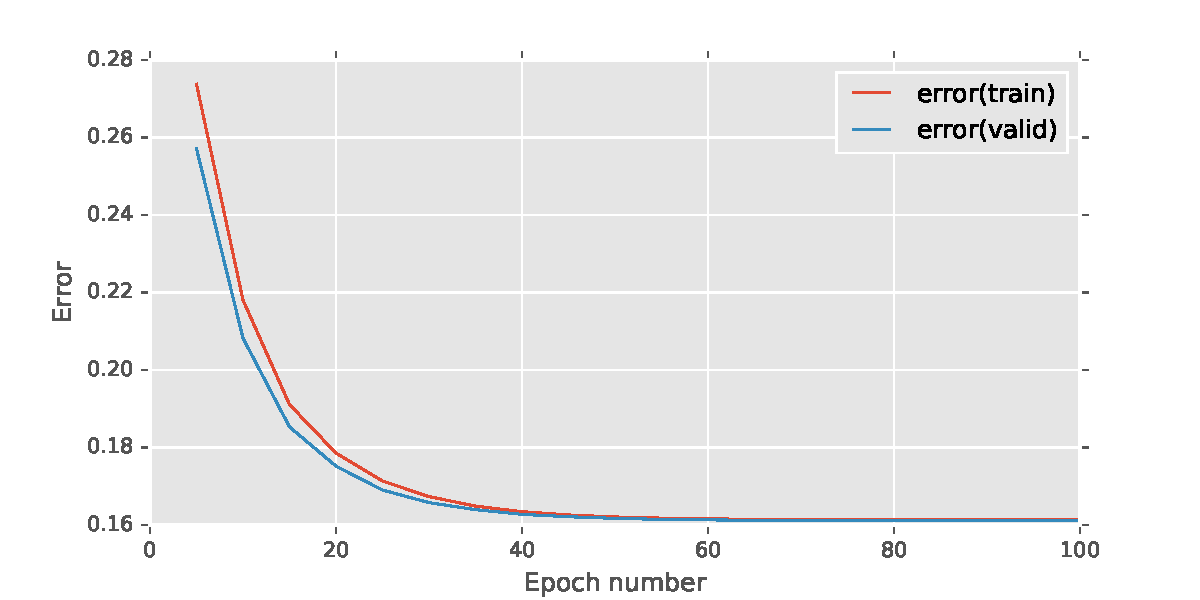
\includegraphics[height=1.5in]{error_with_free_param_10.pdf}
        \caption{error with $r$ = 10}
    \end{subfigure}
	~
    \begin{subfigure}[t]{0.45\textwidth}
        \centering
        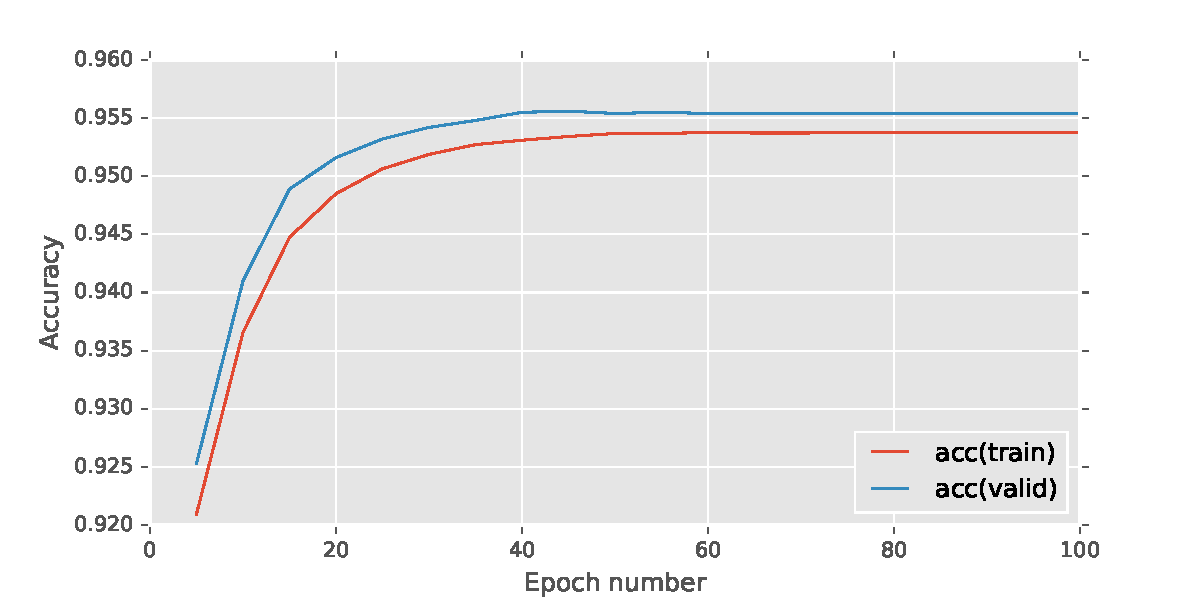
\includegraphics[height=1.5in]{acc_with_param_10.pdf}
        \caption{accuracy with $r$ = 10}
    \end{subfigure}
	~
    \begin{subfigure}[t]{0.45\textwidth}
        \centering
        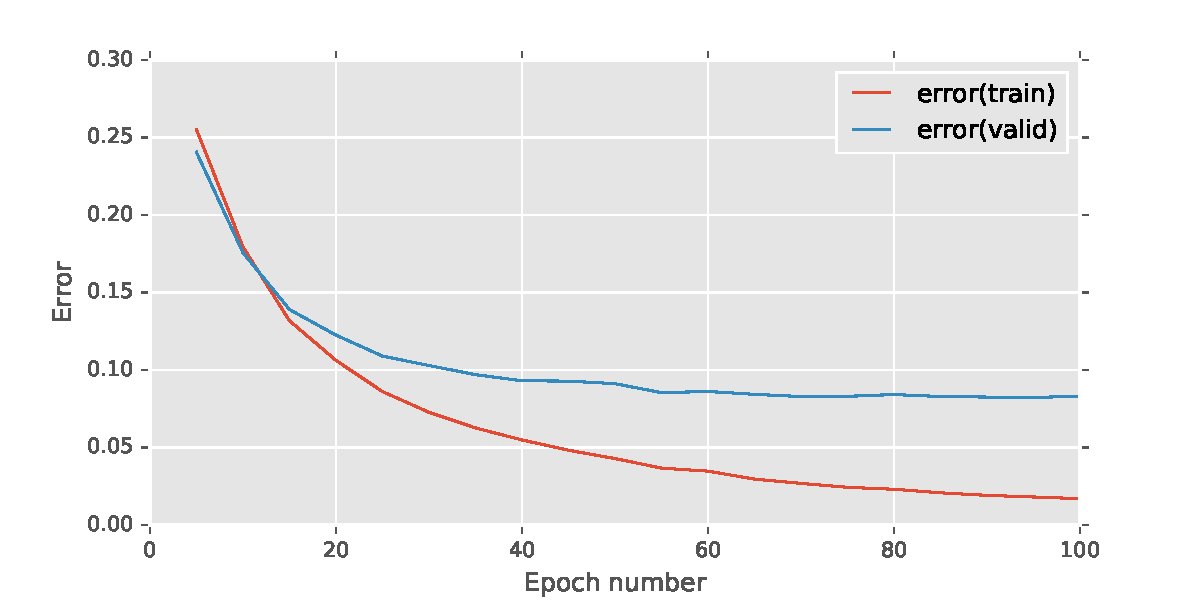
\includegraphics[height=1.5in]{error_with_free_param_100.pdf}
        \caption{error with $r$ = 100}
    \end{subfigure}
	~
    \begin{subfigure}[t]{0.45\textwidth}
        \centering
        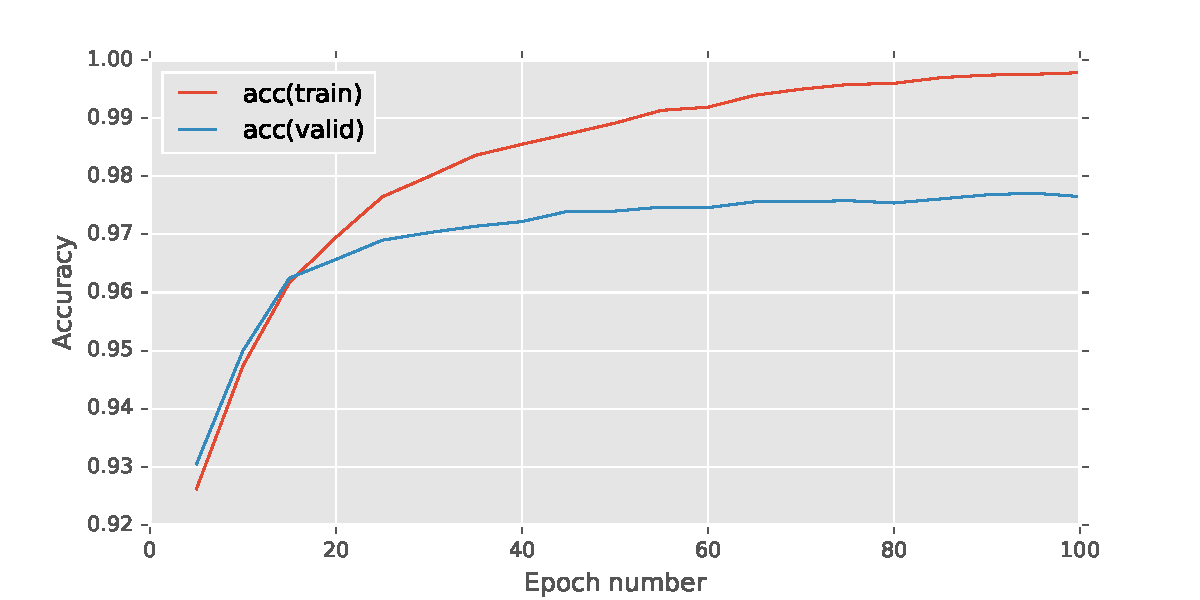
\includegraphics[height=1.5in]{acc_with_param_100.pdf}
        \caption{accuracy with $r$ = 100}
    \end{subfigure}
	~
    \begin{subfigure}[t]{0.45\textwidth}
        \centering
        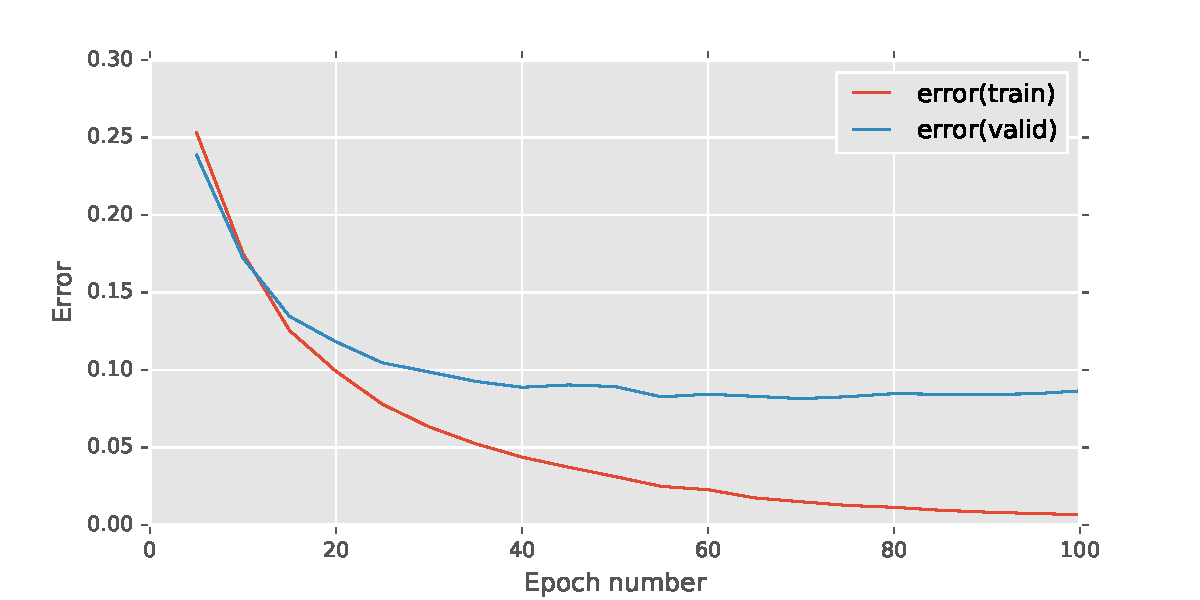
\includegraphics[height=1.5in]{error_with_free_param_1000.pdf}
        \caption{error with $r$ = 1000}
    \end{subfigure}   
    ~
    \begin{subfigure}[t]{0.45\textwidth}
        \centering
        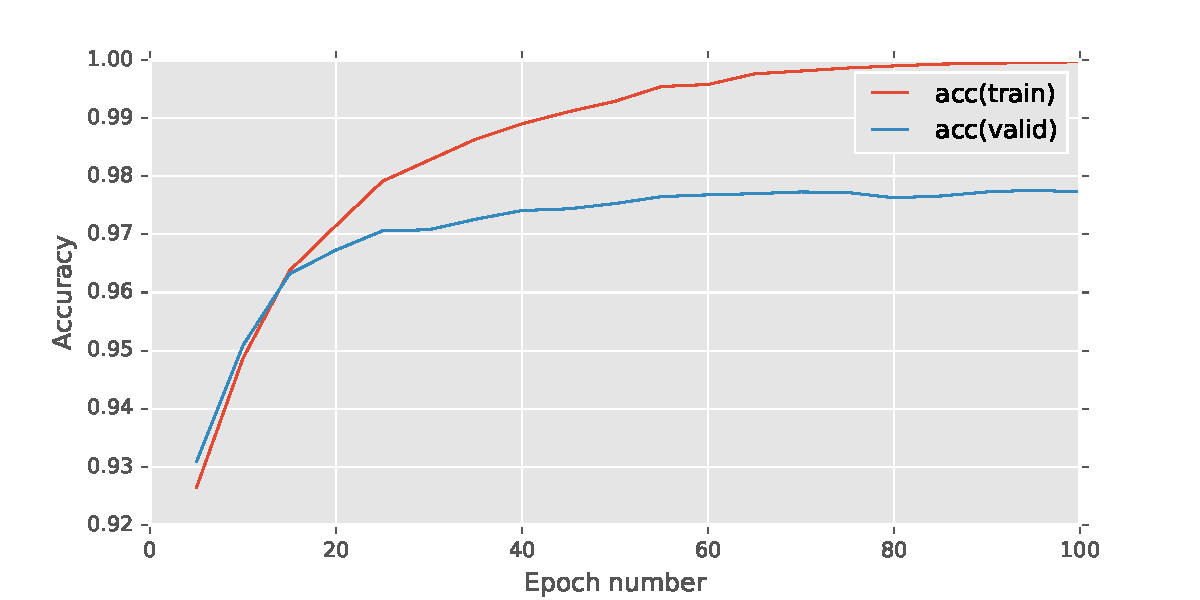
\includegraphics[height=1.5in]{acc_with_param_1000.pdf}
        \caption{accuracy with $r$ = 1000}
    \end{subfigure}    
	~
    \begin{subfigure}[t]{0.45\textwidth}
        \centering
        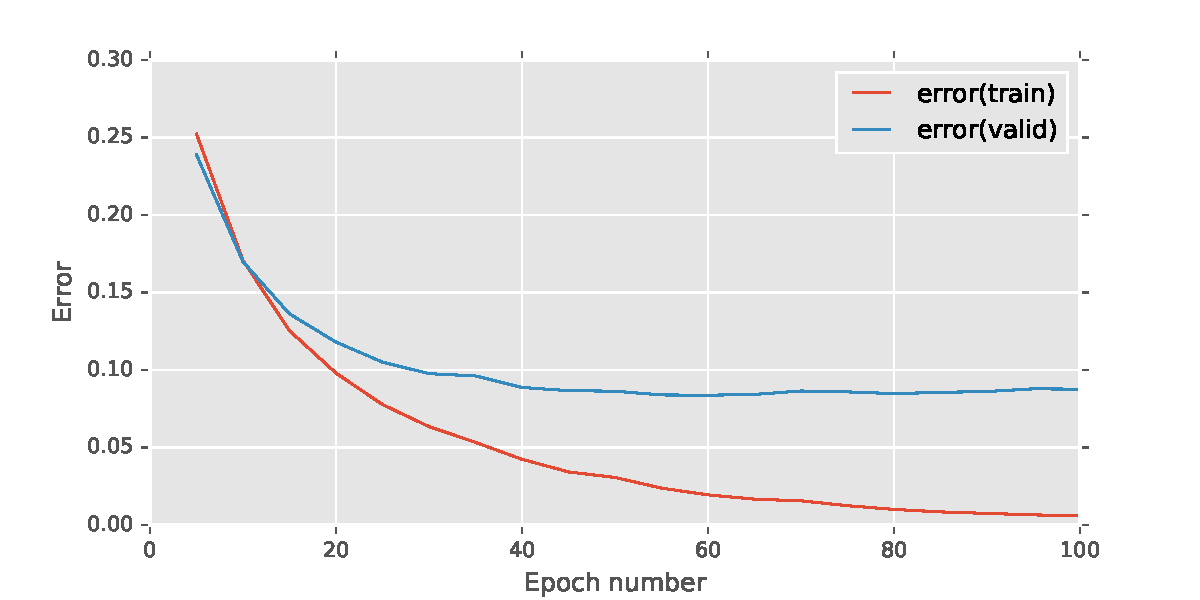
\includegraphics[height=1.5in]{error_with_free_param_10000.pdf}
        \caption{error with $r$ = 10000}
    \end{subfigure}   
    ~
    \begin{subfigure}[t]{0.45\textwidth}
        \centering
        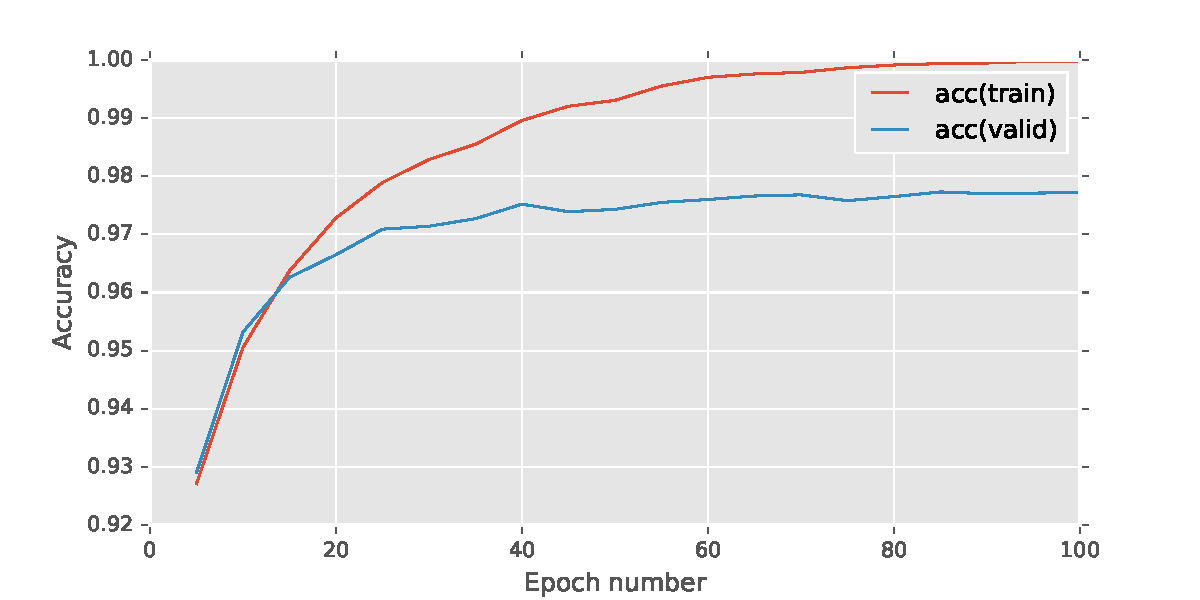
\includegraphics[height=1.5in]{acc_with_param_10000.pdf}
        \caption{accuracy with $r$ = 10000}
    \end{subfigure} 
	~
    \begin{subfigure}[t]{0.45\textwidth}
        \centering
        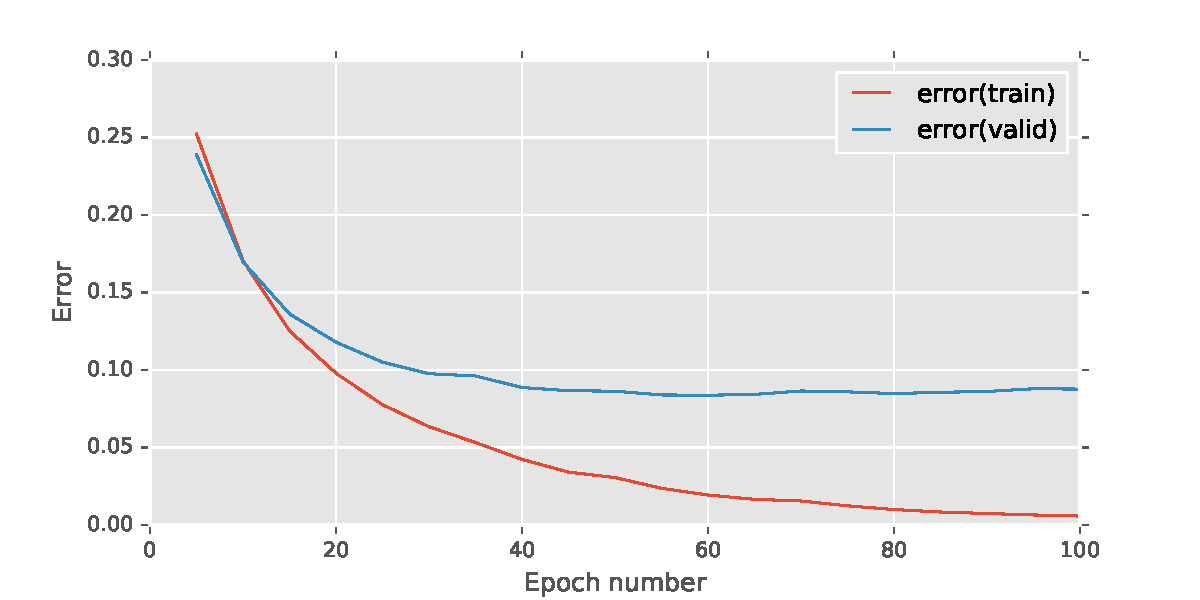
\includegraphics[height=1.5in]{error_with_free_param_50000.pdf}
        \caption{error with $r$ = 50000}
    \end{subfigure}   
    ~
    \begin{subfigure}[t]{0.45\textwidth}
        \centering
        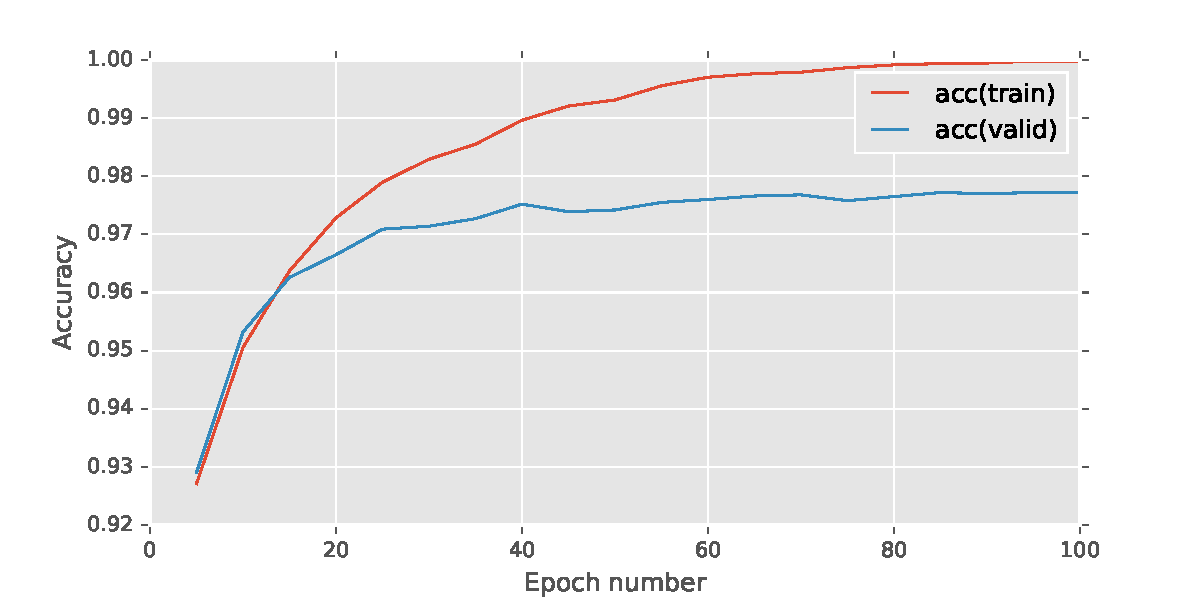
\includegraphics[height=1.5in]{acc_with_param_50000.pdf}
        \caption{accuracy with $r$ = 50000}
    \end{subfigure} 
    \caption{Errors and accuracies with different $r$ when initial learning rate = 0.1}    
    \label{fig:free_param}
\end{figure*}
%Table 1
\begin{table}
\begin{center}
\begin{tabular}{ c c c c c} 
\hline
$r$ & error(train) & error(valid) & acc(train) & acc(valid)\\
\hline
\hline
%0.1& 5.74e-01 & 5.38e-01 & 8.41e-01 & 8.55e-01 \\ 
%1 & 4.14e-01 & 3.86e-01 & 8.88e-01 & 8.95e-01 \\ 
10 & 1.61e-01 & 1.61e-01  &9.54e-01 & 9.55e-01 \\ 
100 &  1.70e-02  & 8.32e-02 & 9.98e-01 & 9.76e-01 \\
1000 &  6.68e-03 & 8.65e-02 & 1.00e+00 & 9.77e-01  \\
1e+04& 5.84e-03 & 8.76e-02 & 1.00e+00 & 9.77e-01 \\
5e+04& 5.78e-03 & 8.77e-02 & 1.00e+00 & 9.77e-01 \\
\end{tabular}
\caption{Performance of different $r$ with initial learning rate = $0.1$}
\label{tb:free_param}
\end{center}	
\end{table}

The performances based on different initial learning rates are given in  Figure.\ref{fig:init_LR}. 
%Figure 2
\begin{figure*}[t!]
    \centering
%    \begin{subfigure}[t]{0.45\textwidth}
%        \centering
%        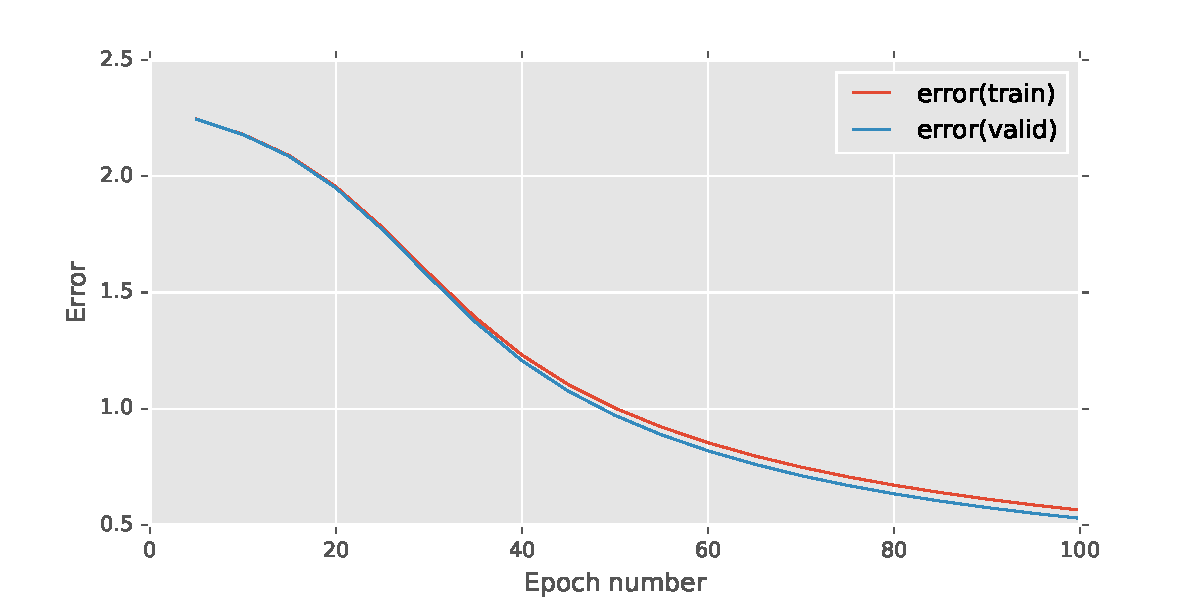
\includegraphics[height=1.5in]{error_with_init_LR_0_001.pdf}
%        \caption{error with initial learning rate = 0.001}
%    \end{subfigure}
%    ~ 
%    \begin{subfigure}[t]{0.45\textwidth}
%        \centering
%        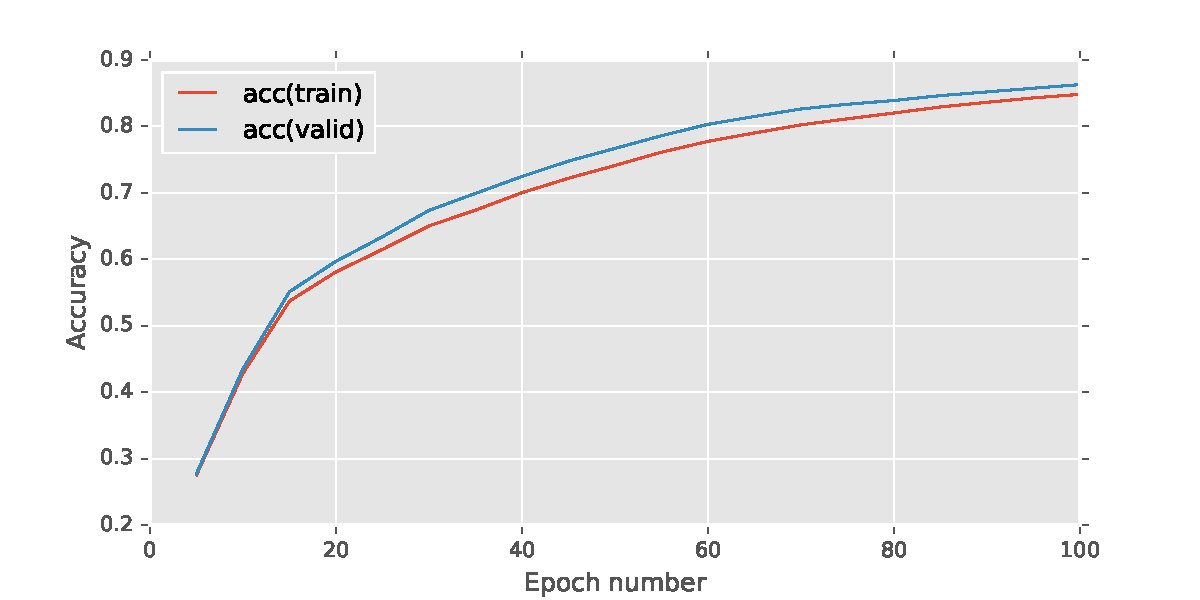
\includegraphics[height=1.5in]{acc_with_init_LR_0_001.pdf}
%        \caption{accuracy with initial learning rate = 0.001}
%    \end{subfigure}
    ~
    \begin{subfigure}[t]{0.45\textwidth}
        \centering
        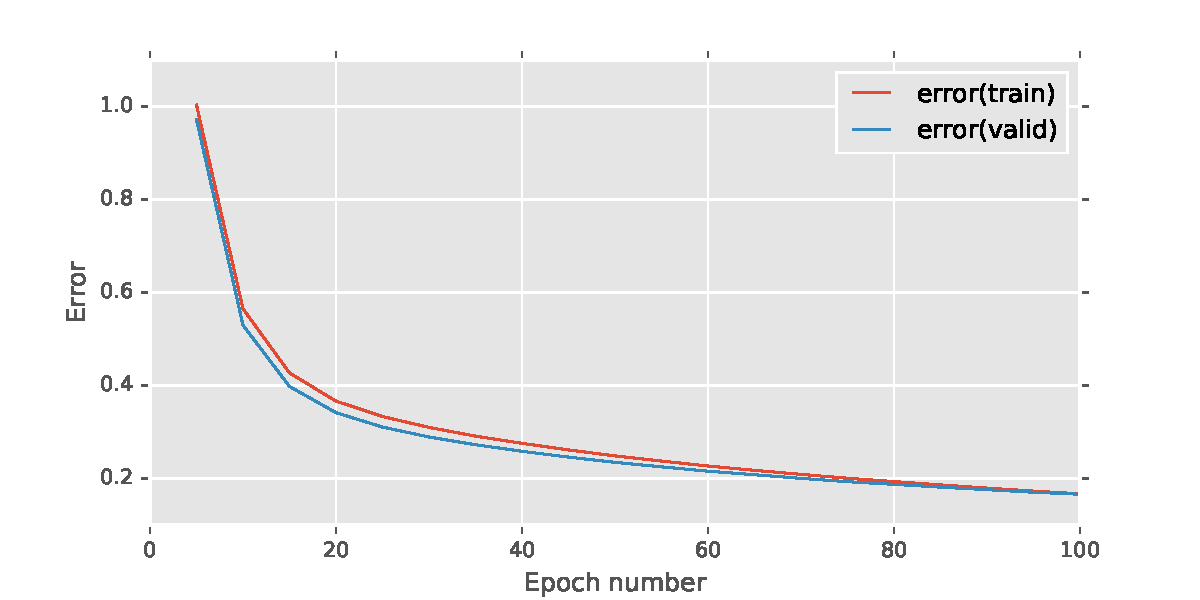
\includegraphics[height=1.5in]{error_with_init_LR_0_01.pdf}
        \caption{error with initial learning rate = 0.01}
    \end{subfigure}
	~
    \begin{subfigure}[t]{0.45\textwidth}
        \centering
        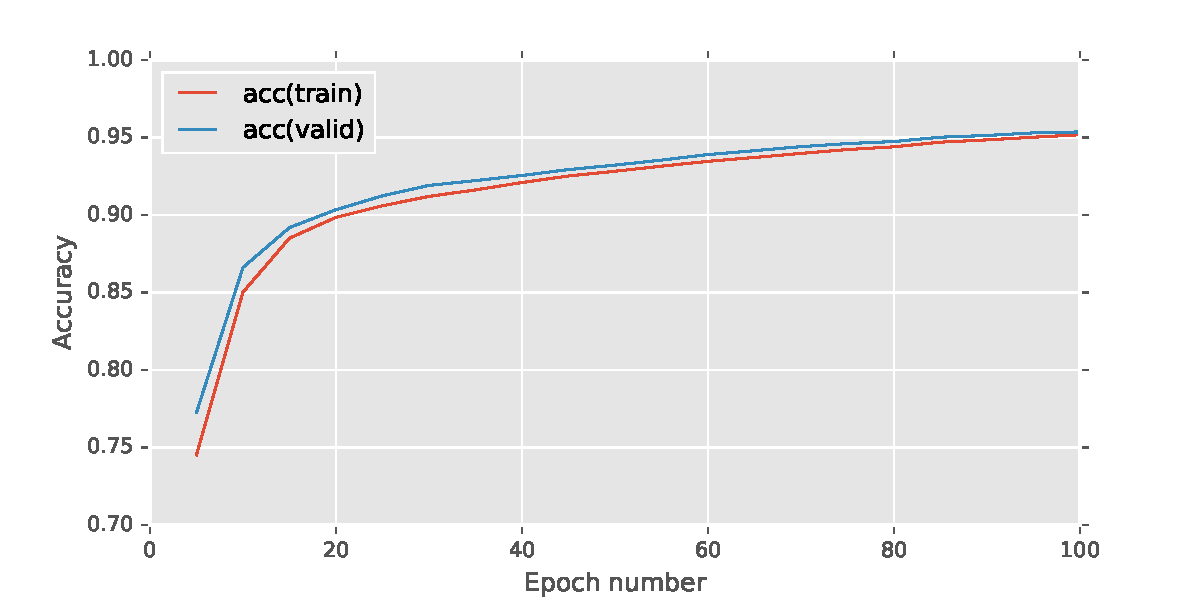
\includegraphics[height=1.5in]{acc_with_init_LR_0_01.pdf}
        \caption{accuracy with initial learning rate = 0.01}
    \end{subfigure}
    ~
    \begin{subfigure}[t]{0.45\textwidth}
        \centering
        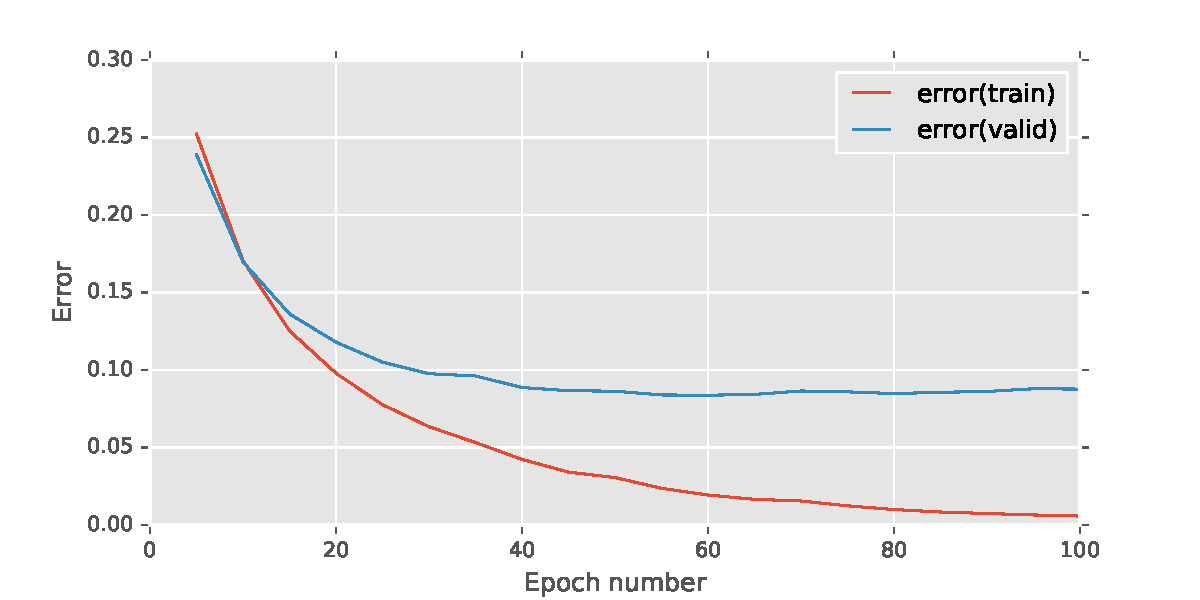
\includegraphics[height=1.5in]{error_with_init_LR_0_1.pdf}
        \caption{error with initial learning rate = 0.1}
    \end{subfigure}
	~
    \begin{subfigure}[t]{0.45\textwidth}
        \centering
        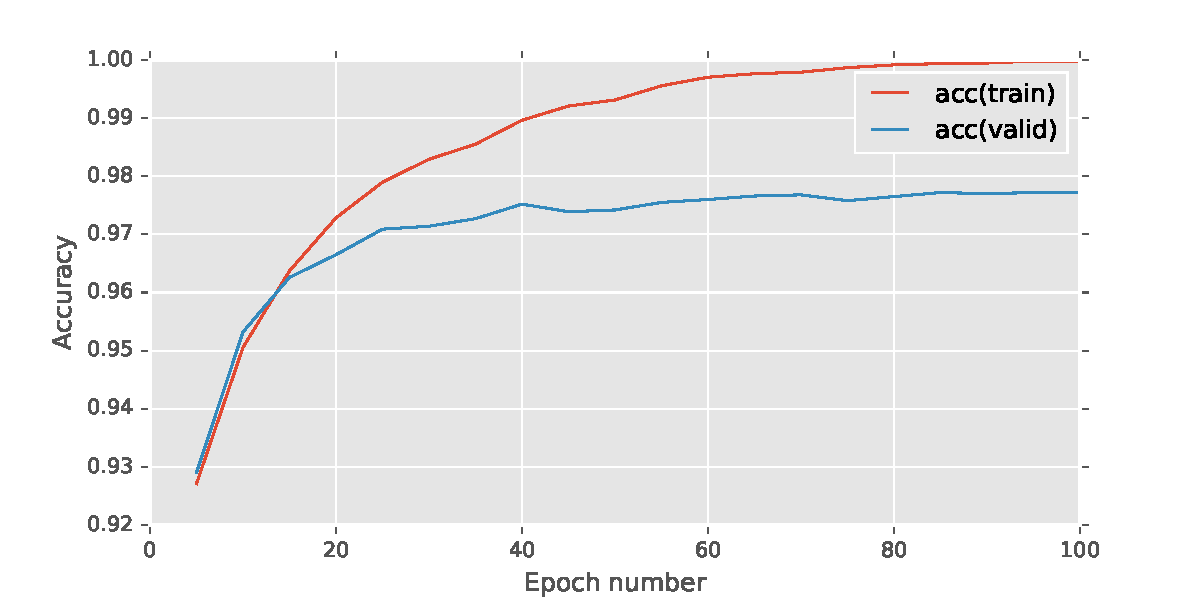
\includegraphics[height=1.5in]{acc_with_init_LR_0_1.pdf}
        \caption{accuracy with initial learning rate = 0.1}
    \end{subfigure}
	~
    \begin{subfigure}[t]{0.45\textwidth}
        \centering
        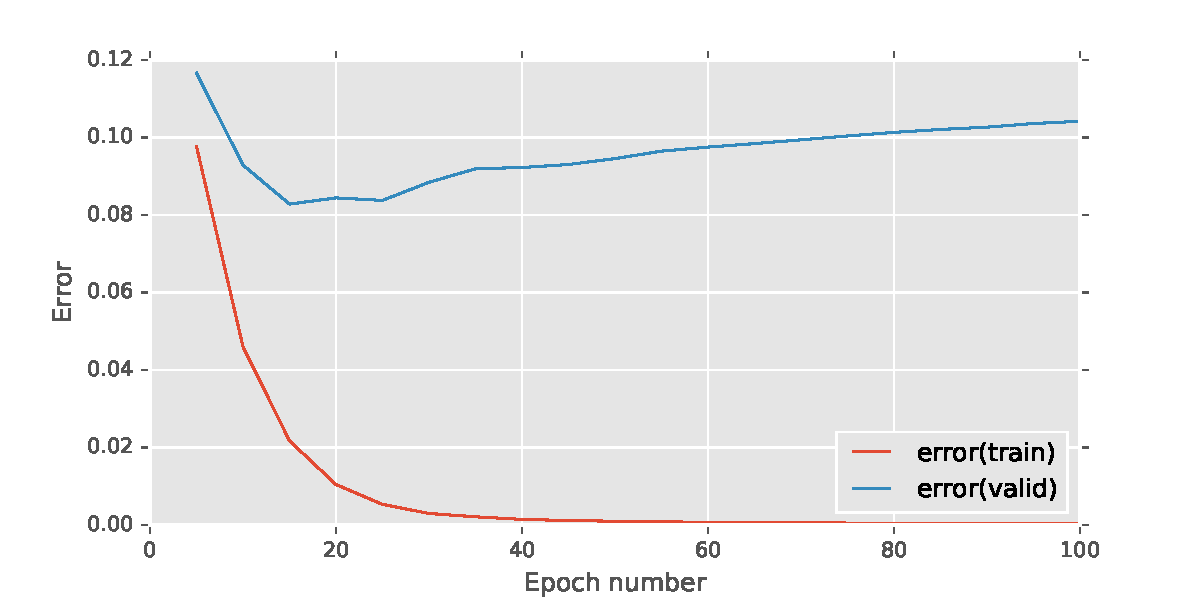
\includegraphics[height=1.5in]{error_with_init_LR_0_5.pdf}
        \caption{error with initial learning rate = 0.5}
    \end{subfigure}
	~
    \begin{subfigure}[t]{0.45\textwidth}
        \centering
        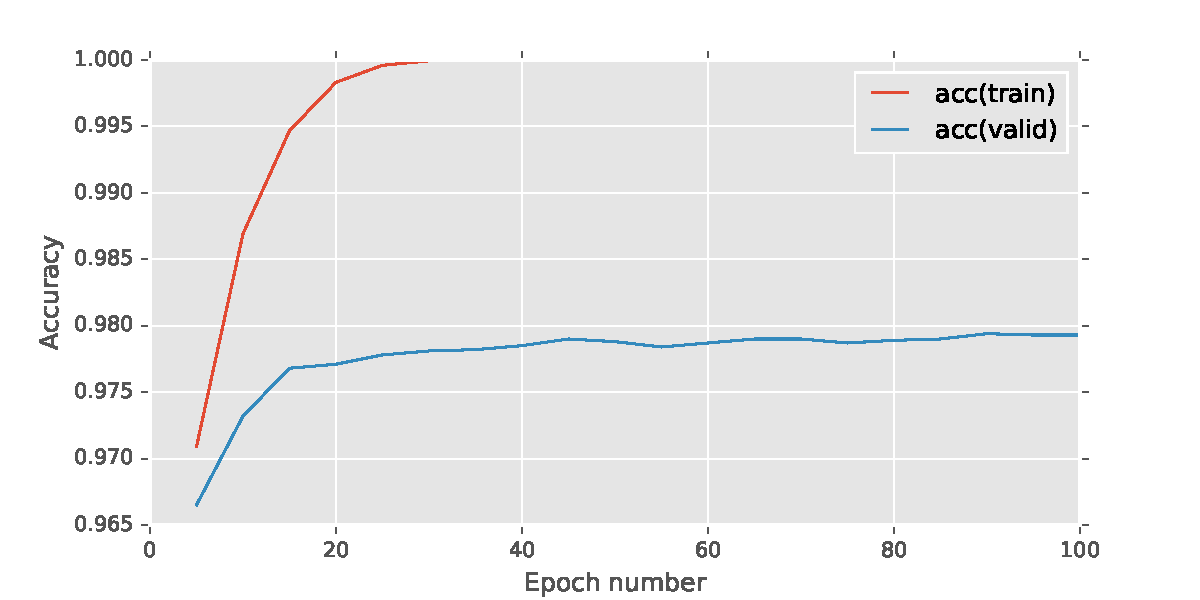
\includegraphics[height=1.5in]{acc_with_init_LR_0_5.pdf}
        \caption{accuracy with initial learning rate = 0.5}
    \end{subfigure}
    ~
    \begin{subfigure}[t]{0.45\textwidth}
        \centering
        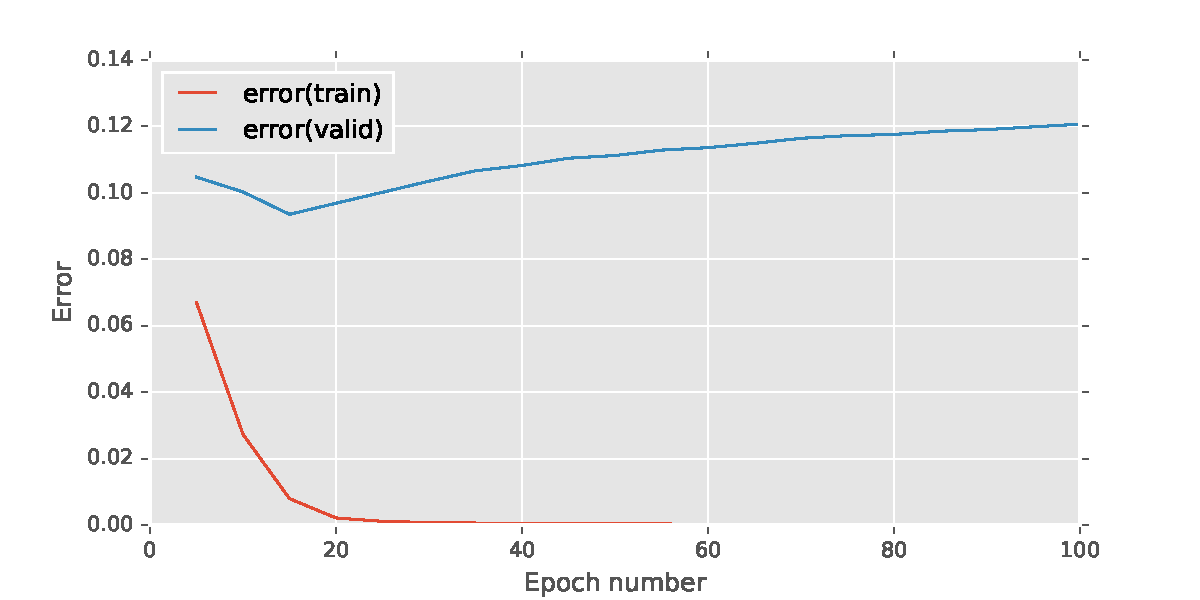
\includegraphics[height=1.5in]{error_with_init_LR_1_0.pdf}
        \caption{error with initial learning rate = 1}
    \end{subfigure}
	~
    \begin{subfigure}[t]{0.45\textwidth}
        \centering
        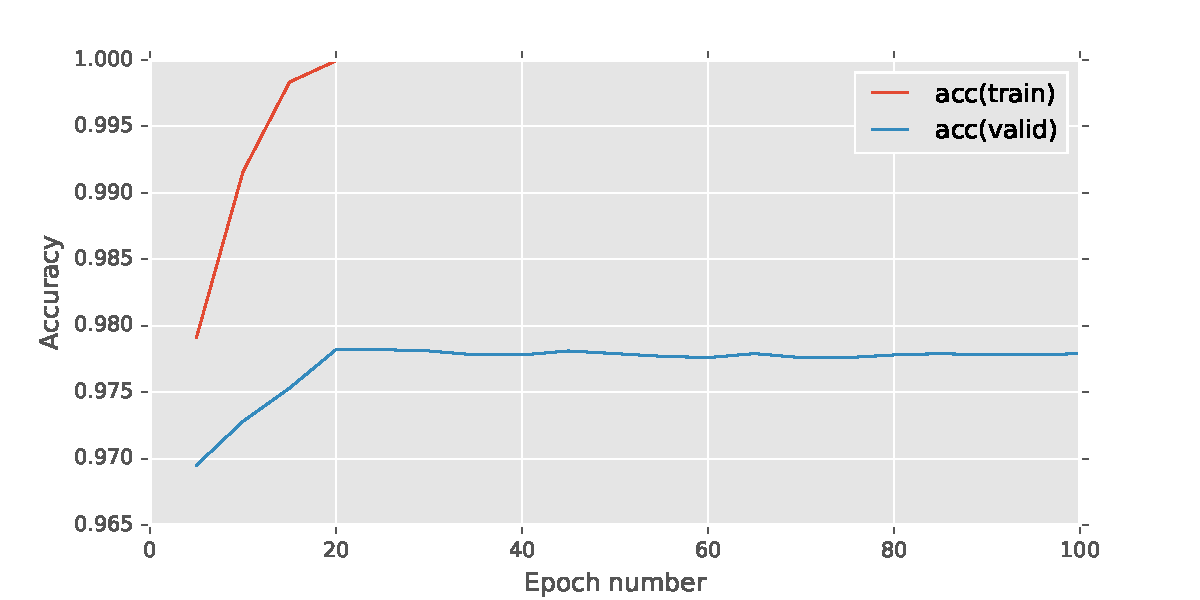
\includegraphics[height=1.5in]{acc_with_init_LR_1_0.pdf}
        \caption{accuracy with initial learning rate = 1}
    \end{subfigure}
	~
    \begin{subfigure}[t]{0.45\textwidth}
        \centering
        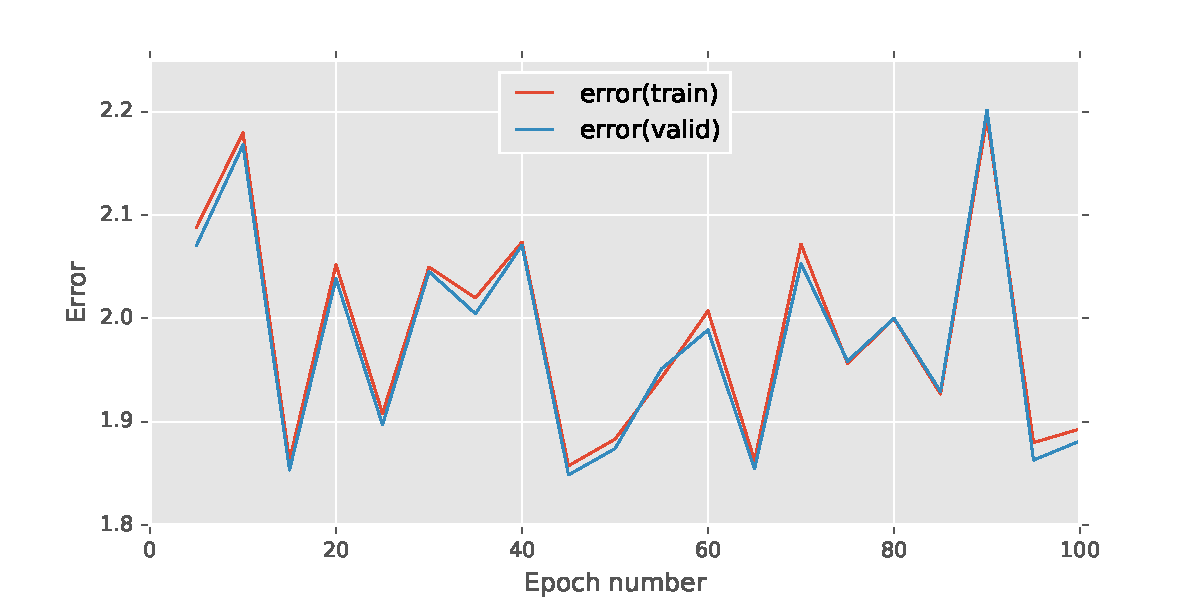
\includegraphics[height=1.5in]{error_with_init_LR_10.pdf}
        \caption{error with initial learning rate = 10}
    \end{subfigure}   
    ~
    \begin{subfigure}[t]{0.45\textwidth}
        \centering
        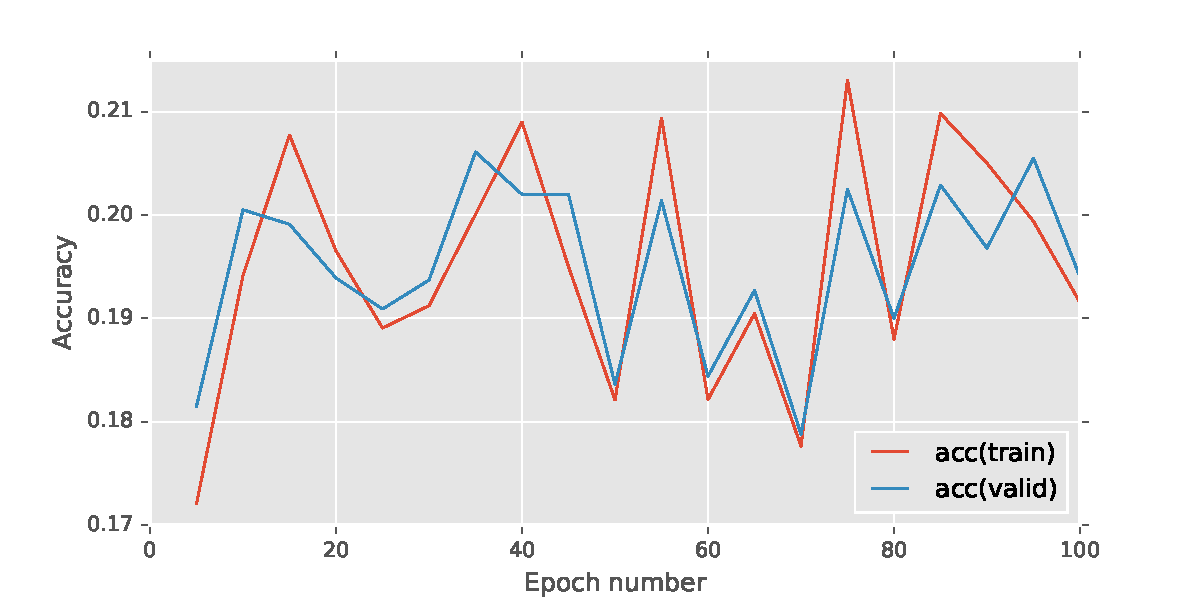
\includegraphics[height=1.5in]{acc_with_init_LR_10.pdf}
        \caption{accuracy with initial learning rate = 10}
    \end{subfigure}    
    \caption{Error and accuracy with different initial learning rates when $r=5e+04$}    
    \label{fig:init_LR}
\end{figure*}

%Table 2
\begin{table}
\begin{center}
\begin{tabular}{ c c c c c} 
\hline
initial learning rate & error(train) & error(valid) & acc(train) & acc(valid)\\
\hline
\hline
0.01& 1.67e-01 & 1.66e-01 & 9.52e-01 & 9.54e-01 \\ 
0.1 & 5.78e-03 & 8.77e-02 & 1.00e+00 & 9.77e-01 \\ 
0.5 & 3.27e-04 & 1.04e-01 & 1.00e+00 & 9.79e-01 \\ 
1  &  1.34e-04  & 1.21e-01 & 1.00e+00 & 9.78e-01 \\
10 &  1.89e+00 & 1.88e+00 & 1.92e-01 & 1.94e-01  \\
\end{tabular}
\caption{Performance of different initial learning rates with $r$ = $10$}
\label{tb:init_lr}
\end{center}	
\end{table}

To compare with the constant learning rate, the results of constant learning rates when the learning rate is set to 0.1 is given in Figure \ref{fig:const_LR}. 

\begin{table}
\begin{center}
\begin{tabular}{ c c c c c} 
\hline
 learning rate type & error(train) & error(valid) & acc(train) & acc(valid)\\
\hline
\hline
const LR = 0.1 & 5.64e-03 & 8.92e-02 &1.00e+00 &9.77e-01\\
TD init\_LR =0.1 \& $r$ = 5e+04 & 5.78e-03 & 8.77e-02 & 1.00e+00 & 9.77e-01 \\ 
\end{tabular}
\caption{Comparison Performance between constant and time-dependent learning rates}
\label{tb:compare_const_td_lr}
\end{center}	
\end{table}

\begin{figure*}[t!]
    \centering
    \begin{subfigure}[t]{0.45\textwidth}
        \centering
        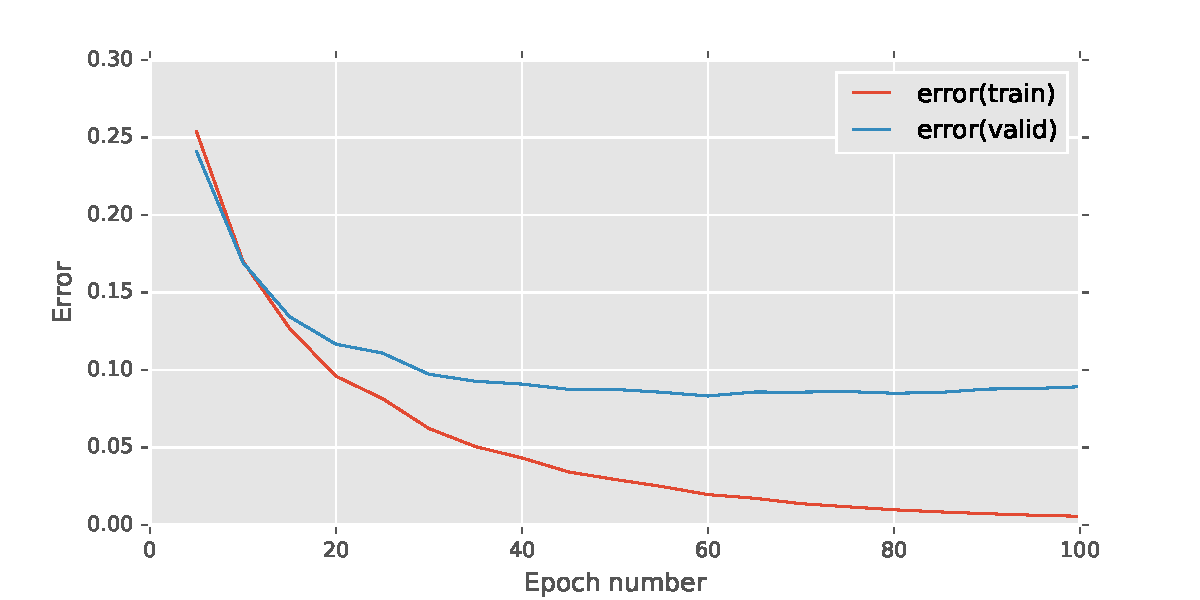
\includegraphics[height=1.5in]{error_with_const_LR_0_1.pdf}
        \caption{error with constant learning rate = 0.1}
    \end{subfigure}   
    ~
    \begin{subfigure}[t]{0.45\textwidth}
        \centering
        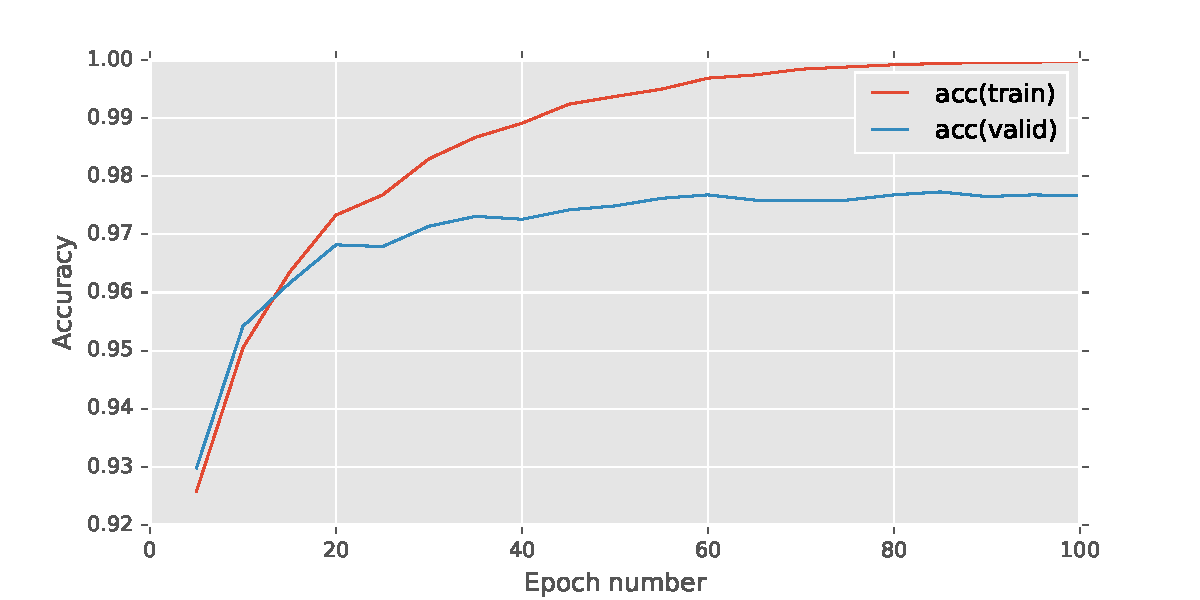
\includegraphics[height=1.5in]{acc_with_const_LR_0_1.pdf}
        \caption{accuracy with initial learning rate = 0.1}
    \end{subfigure}    
    \caption{Error and accuracy with learning rates = 0.1 using gradient descent learning rule}    
    \label{fig:const_LR}
\end{figure*}


\subsection{Discussion and Conclusion}
\subsubsection{Effects of free parameter $r$}
Figure \ref{fig:free_param} indicates that the free parameter $r$ determines how quickly the learning rate decays. larger free parameter converges faster, with higher accuracy. However, smaller free parameter has slower converge speed since the learning rate in each epoch is very small. In summary, larger $r$ results in a better performance and faster convergence.

\subsubsection{Effects of initial learning rate}
From Table \ref{tb:init_lr}, the accuracy is increasing with the increase of initial learning rate except for extremely values such as $10$ because the system becomes more noisy suggesting that the the gradient descent step size is too large. However, the validation error starts to increases when learning rates is over $0.5$. This suggests that the model is overfitting when the initial learning rate is too large. 
\subsubsection{Comparison with constant learning rate}
From Table \ref{tb:compare_const_td_lr}, we can see that the final validation accuracy is similar. However, the time dependent learning rate converges faster than the baseline. Moreover, it has smaller error in validation sets while larger error in training set which means the gap of error between the training and validation sets is smaller in time-dependent learning rates which indicates that the time-dependent learning rats has better performance. 

%----------------------------Section 2------------------------------------------
%----------------------------Section 2------------------------------------------
%----------------------------Section 2------------------------------------------

\newpage
\section{Momentum learning rule}
In this section, a gradient descent learning rule with momentum is investigated.F Firstly, the basic gradient descent learning is compared to the momentum learning rule for several values of the momentum coefficient. Secondly, analogous to the time-dependent learning rate, the time-dependent momentum coefficient is applied and investigated.
\subsection{Methods and Implementation}
\subsubsection{First Task}
In the first task, a for loop is used to test different momentum coefficient. since the momentum coefficient should be in the range of \lbrack 0 1\rbrack, so the 4 figures is chose to compare.
\subsubsection{Second Task}
In the second task, a new schedule is developed according to the following equation.
\begin{equation}
	\alpha(t) = \alpha_\infty (1 - \frac{\gamma}{t + \tau} )
\end{equation}
It is realised in {\bf MomentumCoefficientScheduler} in {\bf mlp.schedulers} with the same interface as the learning rate scheduler. It has three attributes {\bf asy\_mo\_coeff, tau, gamma}, which represent $\alpha_\infty$, $\tau$ and $\gamma$. Also, one method {\bf update\_learning\_rule} which implements the above equation.
In the notebook, a new method called {\bf train\_model\_and\_plot\_stats\_with\_dynamic\_mom\_coeff} is developed to train the model based on the momentum coefficient scheduler. 

The range of $\tau$ to investigate should be limited. If it is much larger than the $\gamma$ and t, the value of momentum coefficient rarely changes which means it becomes another forms of constant momentum coefficient. the value for both $\gamma$ and $\tau$ should not be chosen too small or too large since t is from 1 to 100.
 %----------------------------Results------------------------------------------

\subsection{Results}
\subsubsection{First Task}
The results is shown in Figure \ref{fig:const_mom}. The final error and accuracy rate is shown in the Table \ref{tb:mom}. It indicates that a model with larger momentum coefficient will converge faster than that with smaller momentum coefficient.
%Figure 4
\begin{figure*}[t!]
    \centering
    \begin{subfigure}[t]{0.45\textwidth}
        \centering
        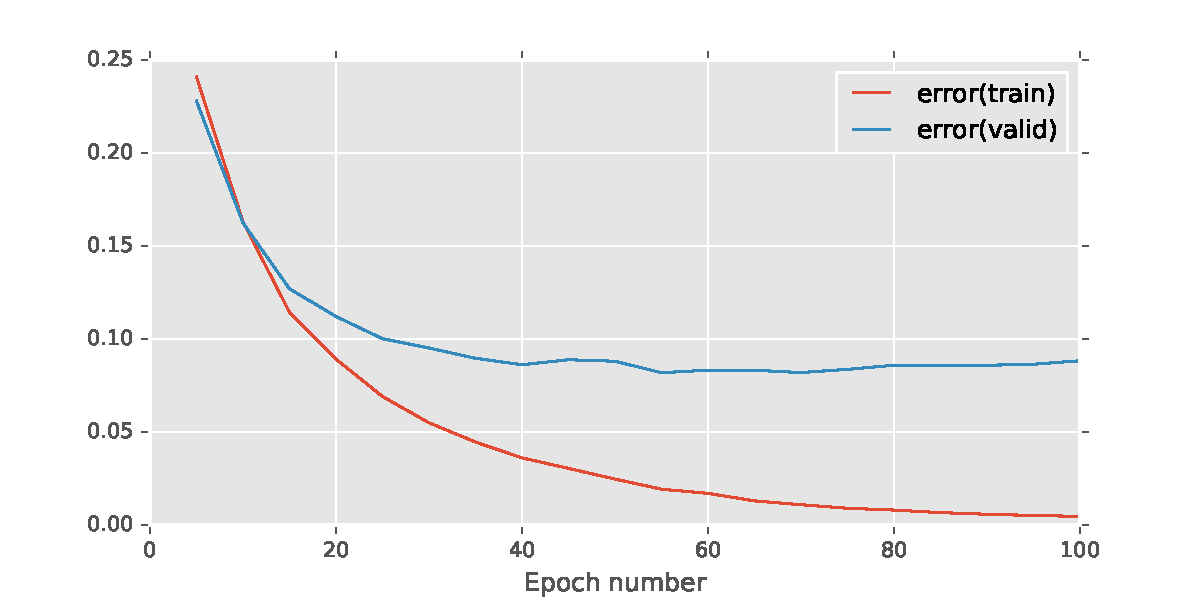
\includegraphics[height=1.5in]{error_with_mom_0_1.pdf}
        \caption{error with momentum coefficient = 0.1}
    \end{subfigure}   
    ~
    \begin{subfigure}[t]{0.45\textwidth}
        \centering
        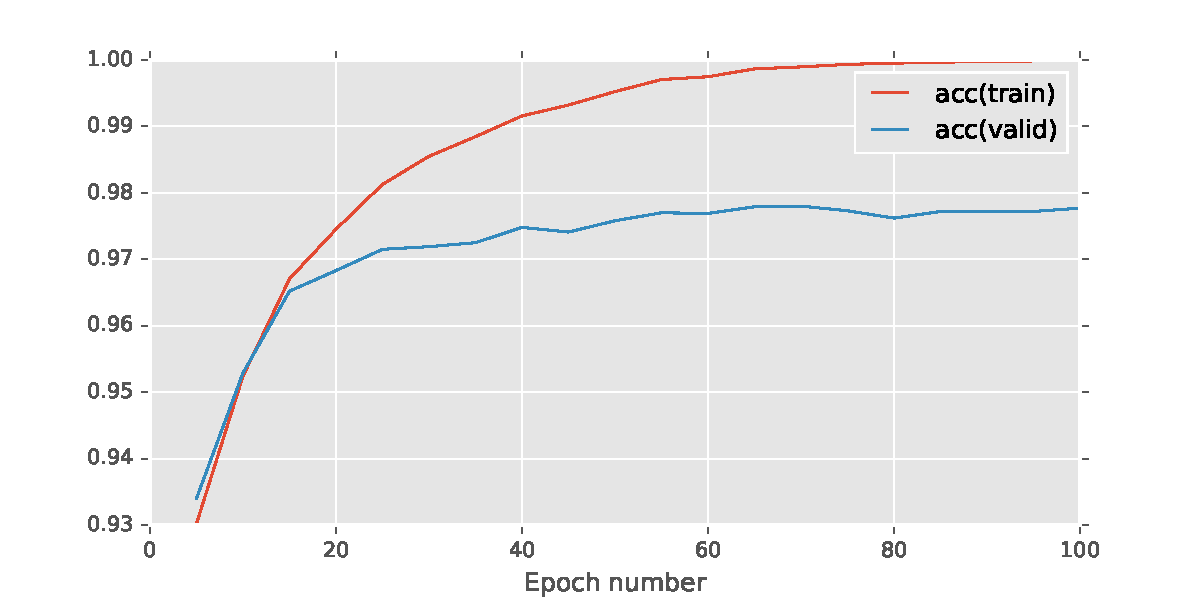
\includegraphics[height=1.5in]{acc_with_mom_0_1.pdf}
        \caption{accuracy with momentum coefficient = 0.1}
    \end{subfigure}   
    ~
    \begin{subfigure}[t]{0.45\textwidth}
        \centering
        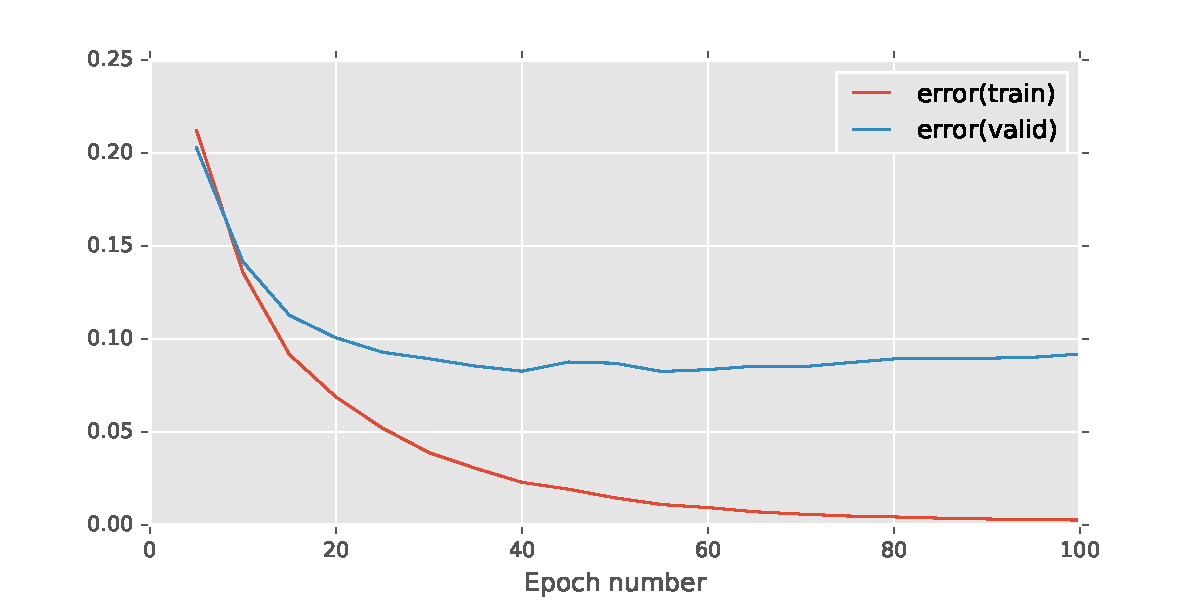
\includegraphics[height=1.5in]{error_with_mom_0_3.pdf}
        \caption{error with momentum coefficient = 0.3}
    \end{subfigure}   
    ~
    \begin{subfigure}[t]{0.45\textwidth}
        \centering
        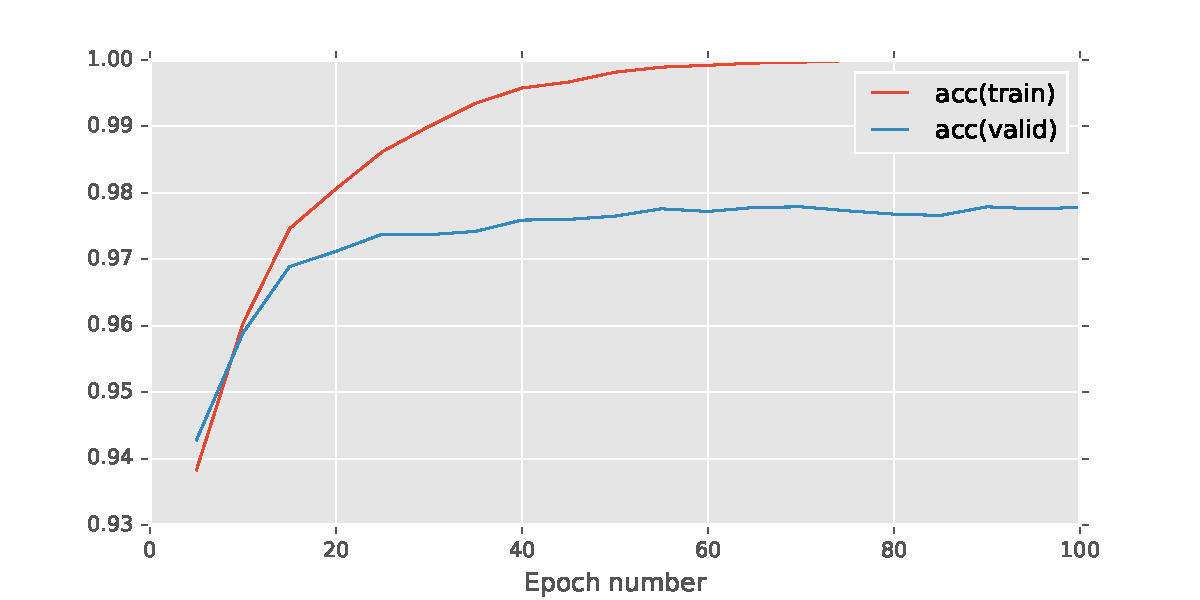
\includegraphics[height=1.5in]{acc_with_mom_0_3.pdf}
        \caption{accuracy with momentum coefficient = 0.3}
    \end{subfigure}    
    ~
    \begin{subfigure}[t]{0.45\textwidth}
        \centering
        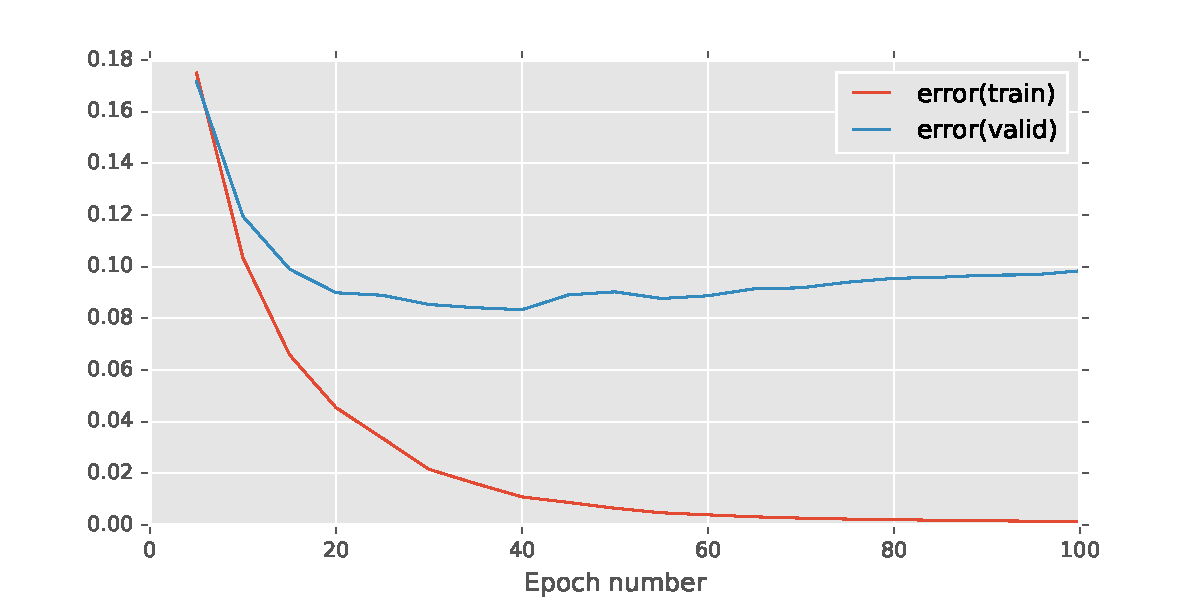
\includegraphics[height=1.5in]{error_with_mom_0_5.pdf}
        \caption{error with momentum coefficient = 0.5}
    \end{subfigure}   
    ~
    \begin{subfigure}[t]{0.45\textwidth}
        \centering
        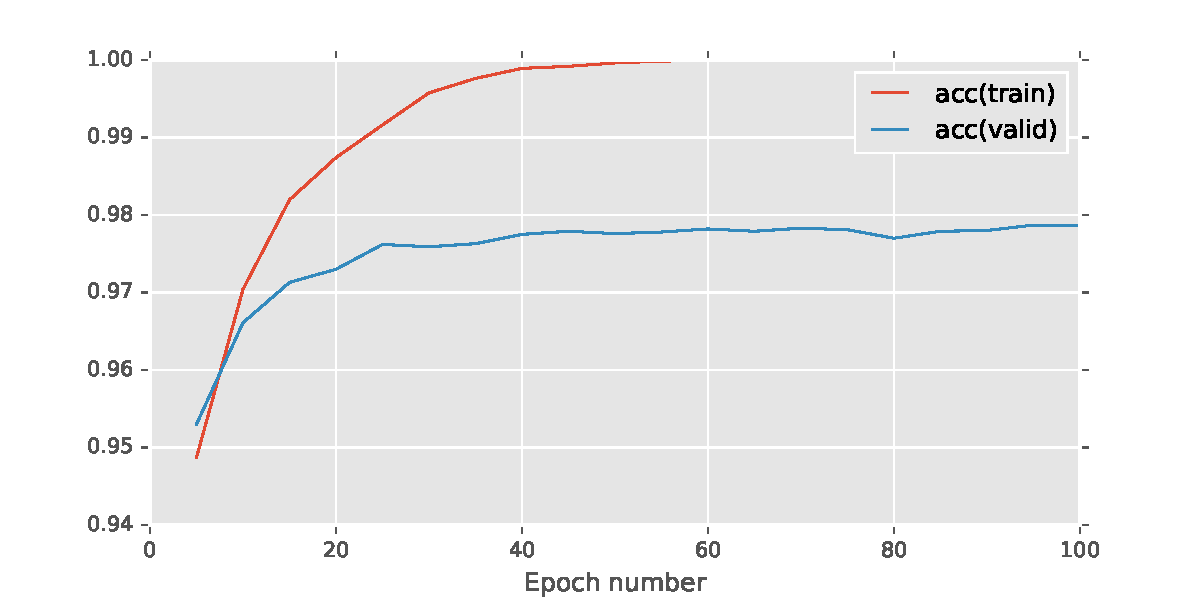
\includegraphics[height=1.5in]{acc_with_mom_0_5.pdf}
        \caption{accuracy with momentum coefficient = 0.5}
    \end{subfigure}      ~
    \begin{subfigure}[t]{0.45\textwidth}
        \centering
        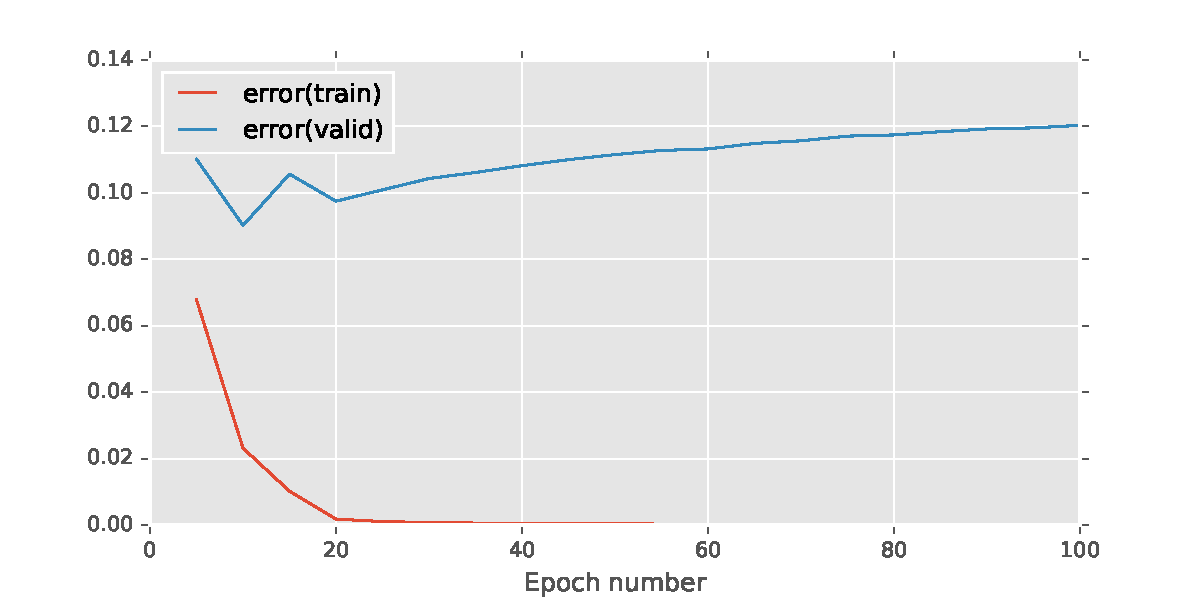
\includegraphics[height=1.5in]{error_with_mom_0_9.pdf}
        \caption{error with momentum coefficient = 0.9}
    \end{subfigure}   
    ~
    \begin{subfigure}[t]{0.45\textwidth}
        \centering
        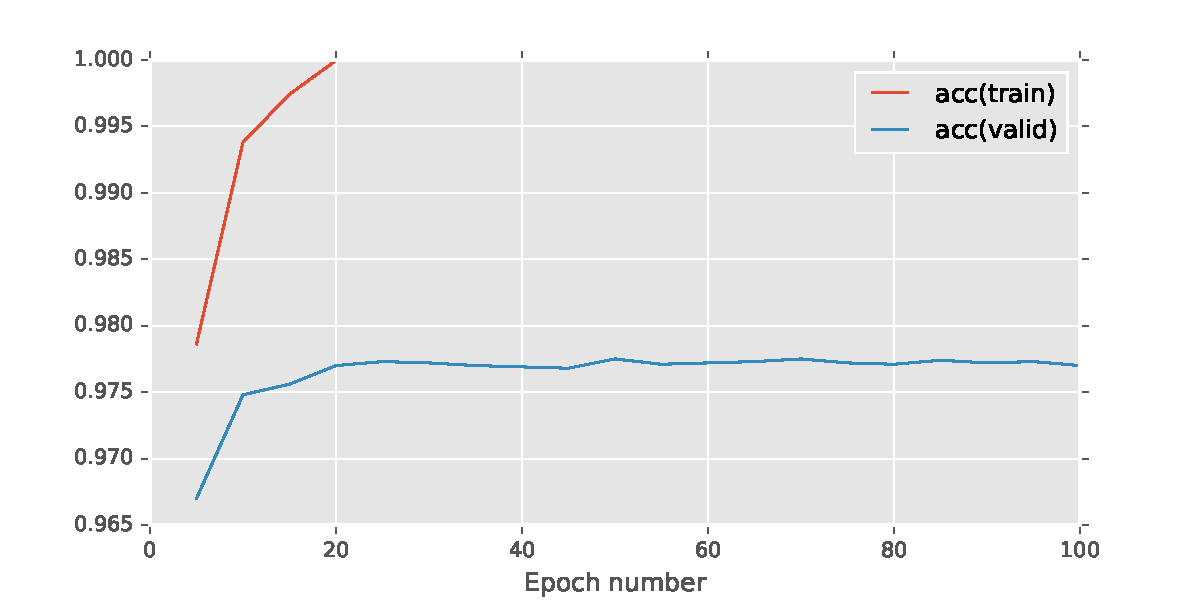
\includegraphics[height=1.5in]{acc_with_mom_0_9.pdf}
        \caption{accuracy with momentum coefficient = 0.9}
    \end{subfigure}      
    \caption{Error and accuracy with different momentum coefficients using momentum learning rule}    
    \label{fig:const_mom}
\end{figure*}

%Table 4
\begin{table}
\begin{center}
\begin{tabular}{ c c c c c} 
\hline
mom\_coeff & error(train) & error(valid) & acc(train) & acc(valid)\\
\hline
\hline
0.1& 4.47e-03 & 8.90e-02 & 1.00 & 0.9775 \\ 
0.3 & 2.56e-03 & 9.25e-02 & 1.00 & 0.9786 \\ 
0.5 & 1.34e-03 & 9.64e-02 & 1.00 & 0.9786 \\ 
0.9  &  1.28e-04  & 1.13e-01 & 1.00 & 0.9787 \\
\end{tabular}
\caption{Performance of different momentum coefficients}
\label{tb:mom}
\end{center}	
\end{table}

\subsubsection{Second Task}
In these parts, three attributes $\alpha_\infty$, $\tau$ and $\gamma$ are investigated for different values. The results is given by Figure \ref{fig:asy_mom}. \ref{fig:tau}. and \ref{fig:gamma}. The final performance is shown in Table \ref{fig:asy_mom}. \ref{fig:tau}. and \ref{fig:gamma}.

\begin{figure*}[t!]
    \centering
    \begin{subfigure}[t]{0.45\textwidth}
        \centering
        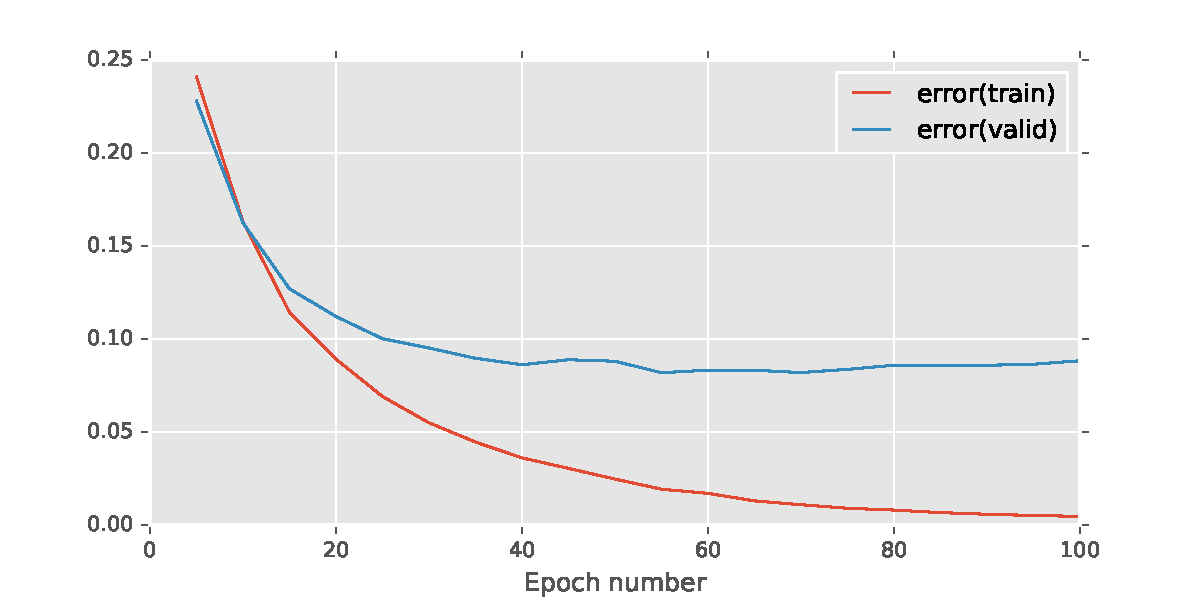
\includegraphics[height=1.5in]{error_with_asy_mom_0_1.pdf}
        \caption{error with asym\_mom\_coeff = 0.1}
    \end{subfigure}   
    ~
    \begin{subfigure}[t]{0.45\textwidth}
        \centering
        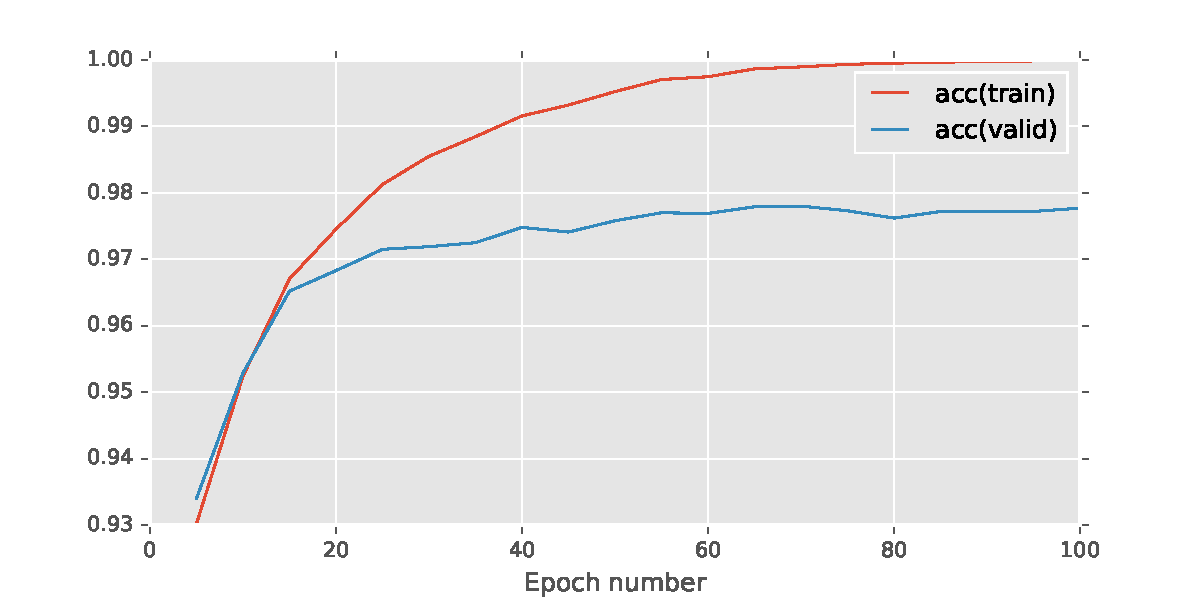
\includegraphics[height=1.5in]{acc_with_asy_mom_0_1.pdf}
        \caption{accuracy with asym\_mom\_coeff = 0.1}
    \end{subfigure}
    ~ 
    \begin{subfigure}[t]{0.45\textwidth}
        \centering
        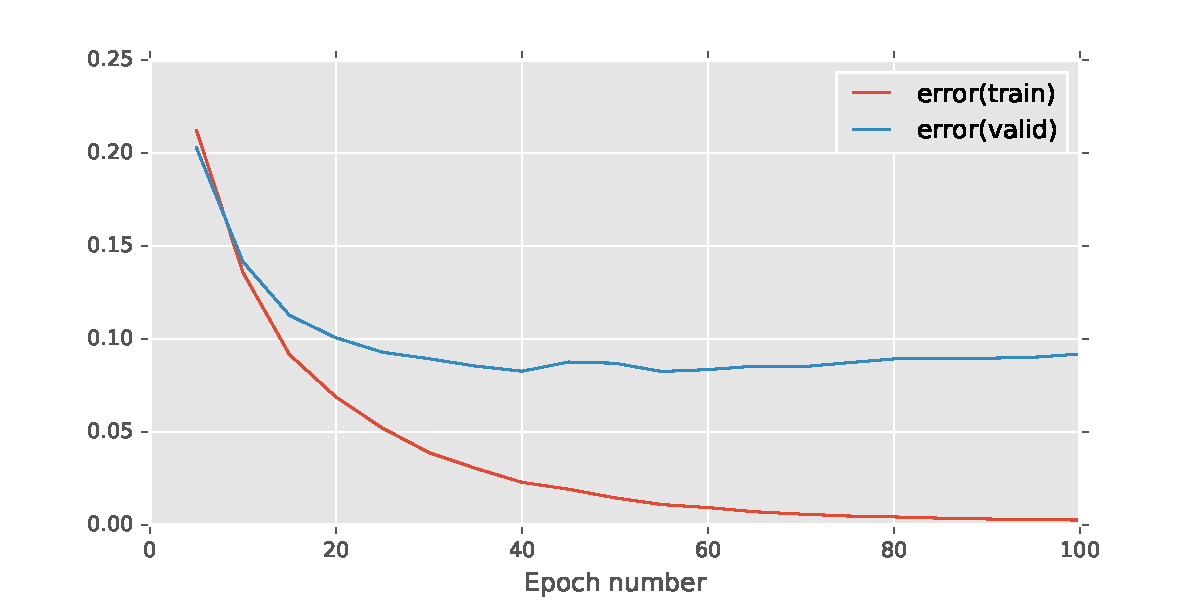
\includegraphics[height=1.5in]{error_with_asy_mom_0_3.pdf}
        \caption{error with asym\_mom\_coeff = 0.3}
    \end{subfigure}   
    ~
    \begin{subfigure}[t]{0.45\textwidth}
        \centering
        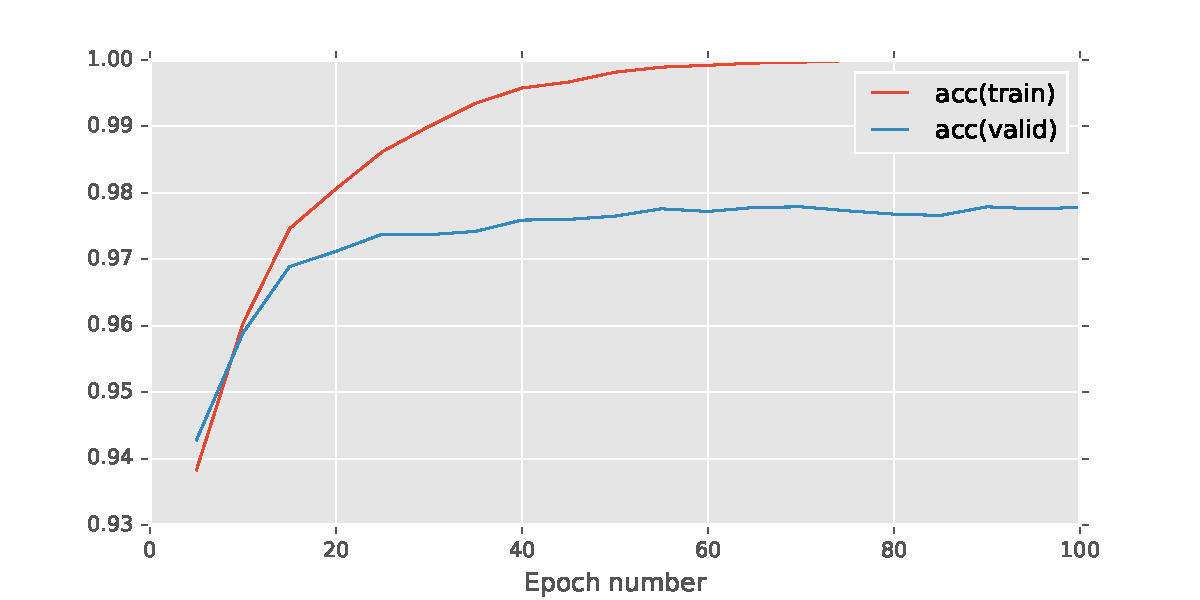
\includegraphics[height=1.5in]{acc_with_asy_mom_0_3.pdf}
        \caption{accuracy with asym\_mom\_coeff = 0.3}
    \end{subfigure}
    ~ 
    \begin{subfigure}[t]{0.45\textwidth}
        \centering
        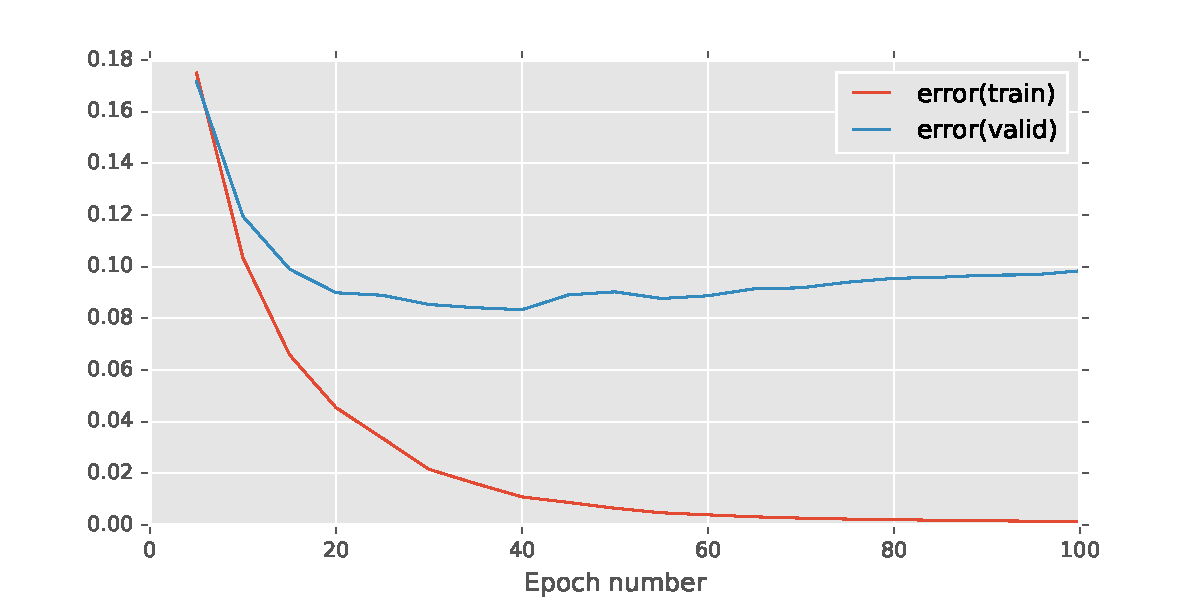
\includegraphics[height=1.5in]{error_with_asy_mom_0_5.pdf}
        \caption{error with asym\_mom\_coeff = 0.5}
    \end{subfigure}   
    ~
    \begin{subfigure}[t]{0.45\textwidth}
        \centering
        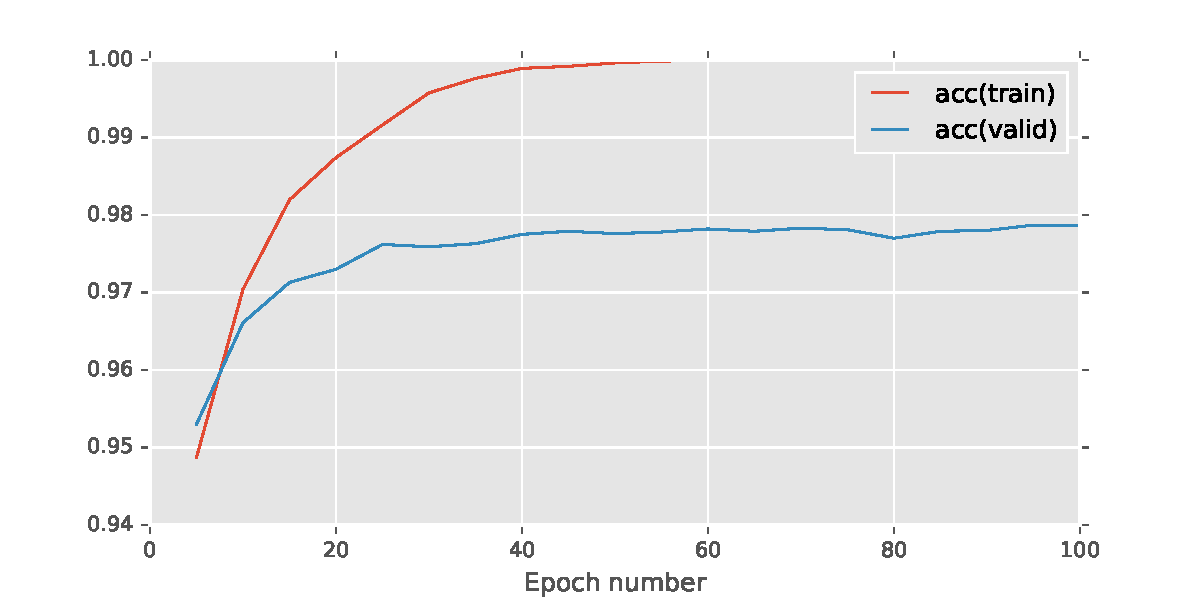
\includegraphics[height=1.5in]{acc_with_asy_mom_0_5.pdf}
        \caption{accuracy with asym\_mom\_coeff = 0.5}
    \end{subfigure}
    ~ 
    \begin{subfigure}[t]{0.45\textwidth}
        \centering
        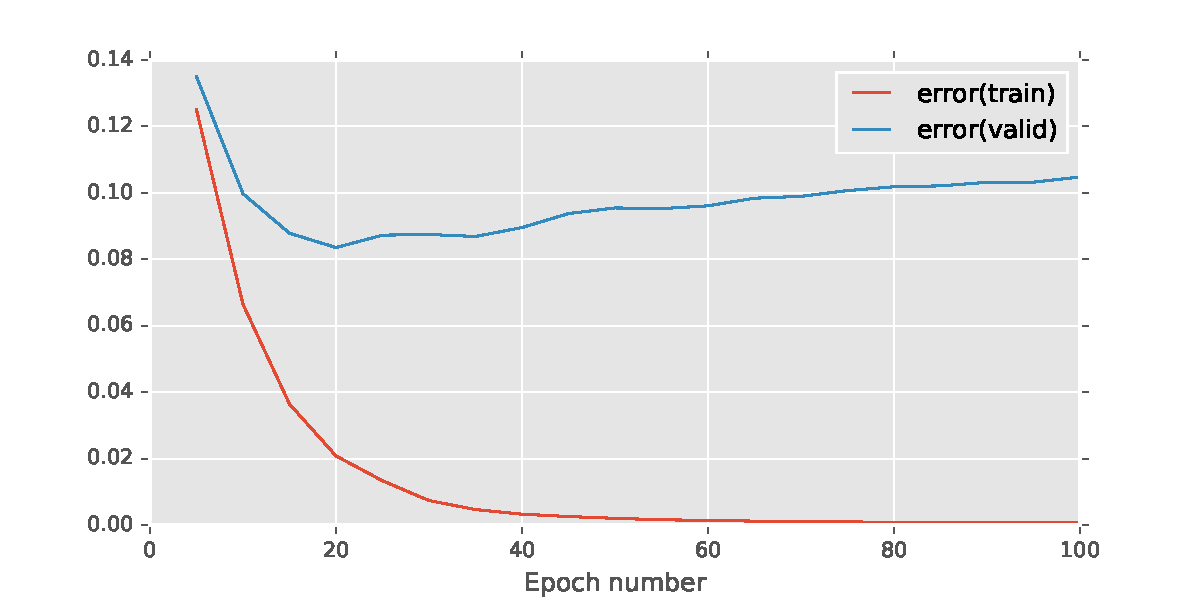
\includegraphics[height=1.5in]{error_with_asy_mom_0_7.pdf}
        \caption{error with asym\_mom\_coeff = 0.7}
    \end{subfigure}   
    ~
    \begin{subfigure}[t]{0.45\textwidth}
        \centering
        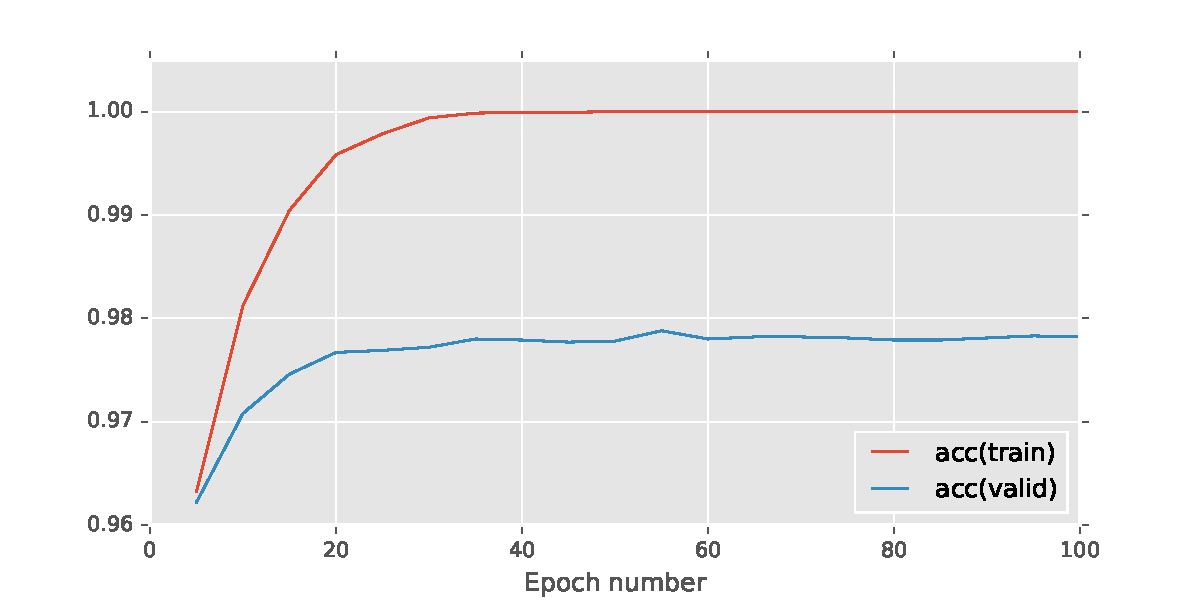
\includegraphics[height=1.5in]{acc_with_asy_mom_0_7.pdf}
        \caption{accuracy with asym\_mom\_coeff = 0.7}
    \end{subfigure}
    ~ 
    \begin{subfigure}[t]{0.45\textwidth}
        \centering
        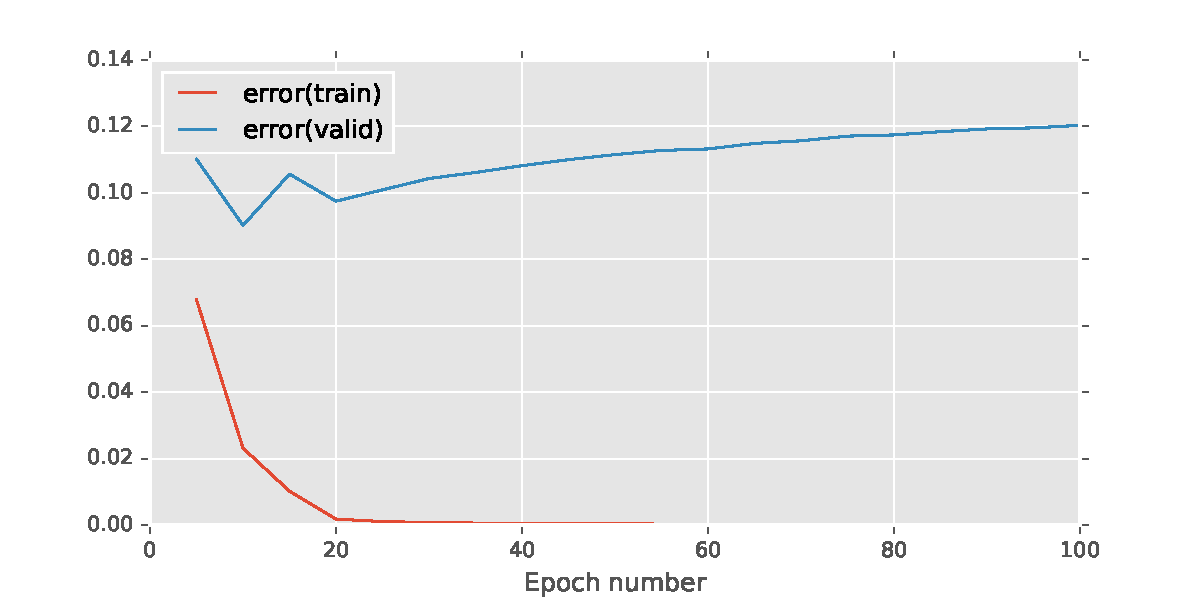
\includegraphics[height=1.5in]{error_with_asy_mom_0_9.pdf}
        \caption{error with asym\_mom\_coeff = 0.9}
    \end{subfigure}   
    ~
    \begin{subfigure}[t]{0.45\textwidth}
        \centering
        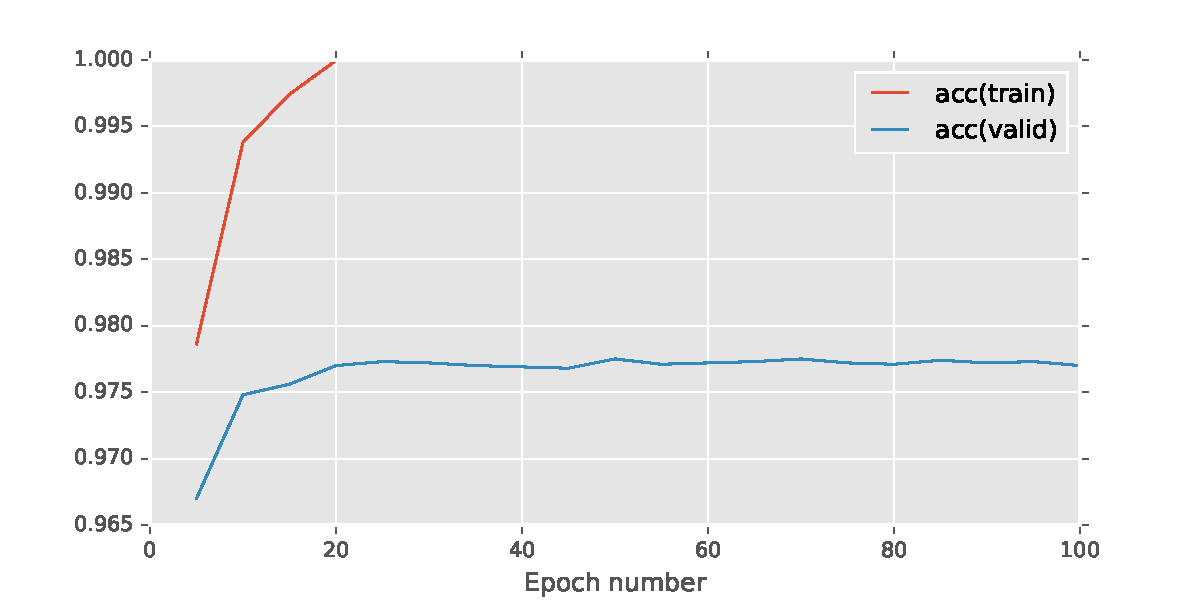
\includegraphics[height=1.5in]{acc_with_asy_mom_0_9.pdf}
        \caption{accuracy with asym\_mom\_coeff = 0.9}
    \end{subfigure}
    \caption{Error and accuracy with several asymptotic momentum coefficients using momentum coefficient scheduler}    
    \label{fig:asy_mom}
\end{figure*}


%Table 5
\begin{table}
\begin{center}
\begin{tabular}{ c c c c c} 
\hline
asy\_mom\_coeff & error(train) & error(valid) & acc(train) & acc(valid)\\
\hline
\hline
0.1& 4.47e-03 & 8.90e-02 & 1.00 & 0.9775 \\ 
0.3 & 2.56e-03 & 9.25e-02 & 1.00 & 0.9786 \\ 
0.5 & 1.34e-03 & 9.64e-02 & 1.00 & 0.9786 \\ 
0.7 & 5.83-04 & 1.02e-01 & 1.00 & 0.9783 \\
0.9  &  1.28e-04 & 1.13-e01 & 1.00 & 0.9787 \\
\end{tabular}
\caption{Performance of different asymptotic momentum coefficients with $\gamma = 1$, $tau=2$}
\label{tb:asy_mom}
\end{center}	
\end{table}

%Table 6
\begin{table}
\begin{center}
\begin{tabular}{ c c c c c} 
\hline
$\tau$ & error(train) & error(valid) & acc(train) & acc(valid)\\
\hline
\hline
1.0& 1.71e-04 & 1.14e-01 & 1.00 & 0.9787 \\ 
2.0& 1.68e-04 & 1.10e-01 & 1.00 & 0.9804 \\ 
5.0& 1.65e-04 & 1.08e-01 & 1.00 &  0.9801\\ 
10.0& 1.59e-04 & 1.10e-01 & 1.00 & 0.9791 \\
100.0&  1.39e-04 & 1.13-e01 & 1.00 & 0.9795 \\
\end{tabular}
\caption{Performance of different $\tau$ with $\gamma = 1.0$ and asy\_mom\_coeff = 0.9}
\label{tb:tau}
\end{center}	
\end{table}
\begin{figure*}[t!]
    \centering
    \begin{subfigure}[t]{0.45\textwidth}
        \centering
        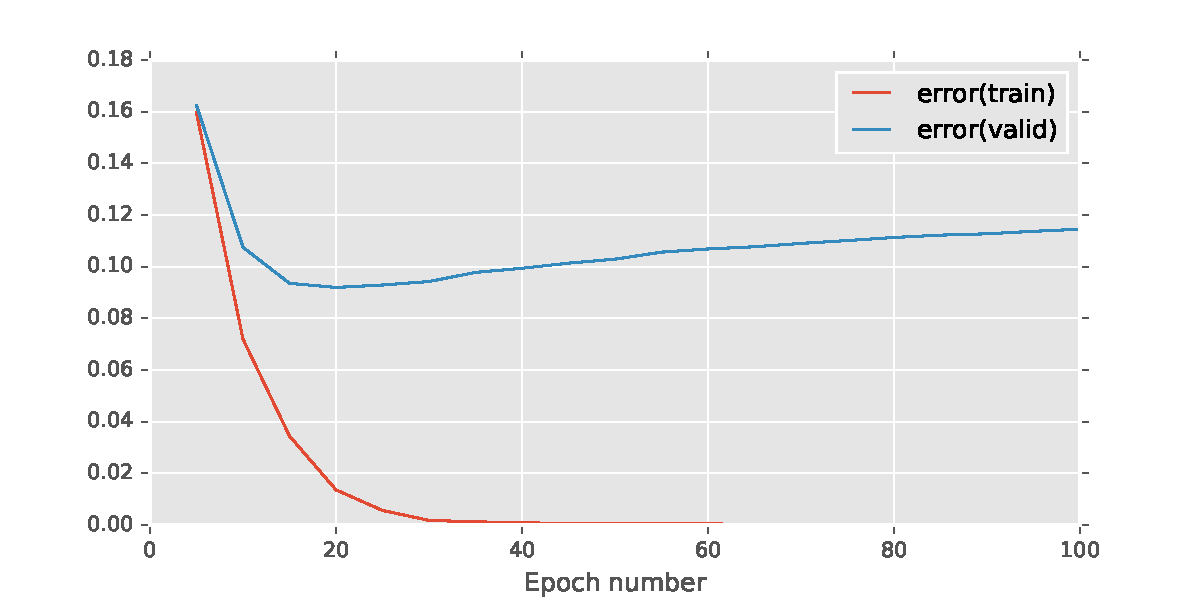
\includegraphics[height=1.5in]{error_with_tau_1_0.pdf}
        \caption{error with $\tau$ = 1.0}
    \end{subfigure}   
    ~
    \begin{subfigure}[t]{0.45\textwidth}
        \centering
        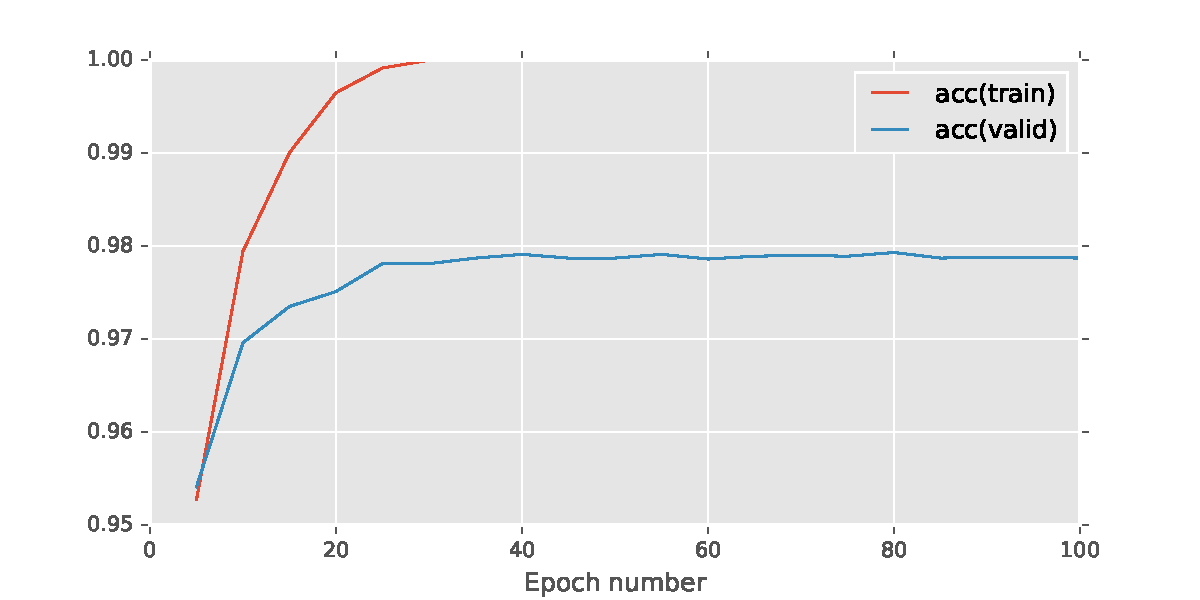
\includegraphics[height=1.5in]{acc_with_tau_1_0.pdf}
        \caption{accuracy with $\tau$ = 1.0}
    \end{subfigure}   
    ~
    \begin{subfigure}[t]{0.45\textwidth}
        \centering
        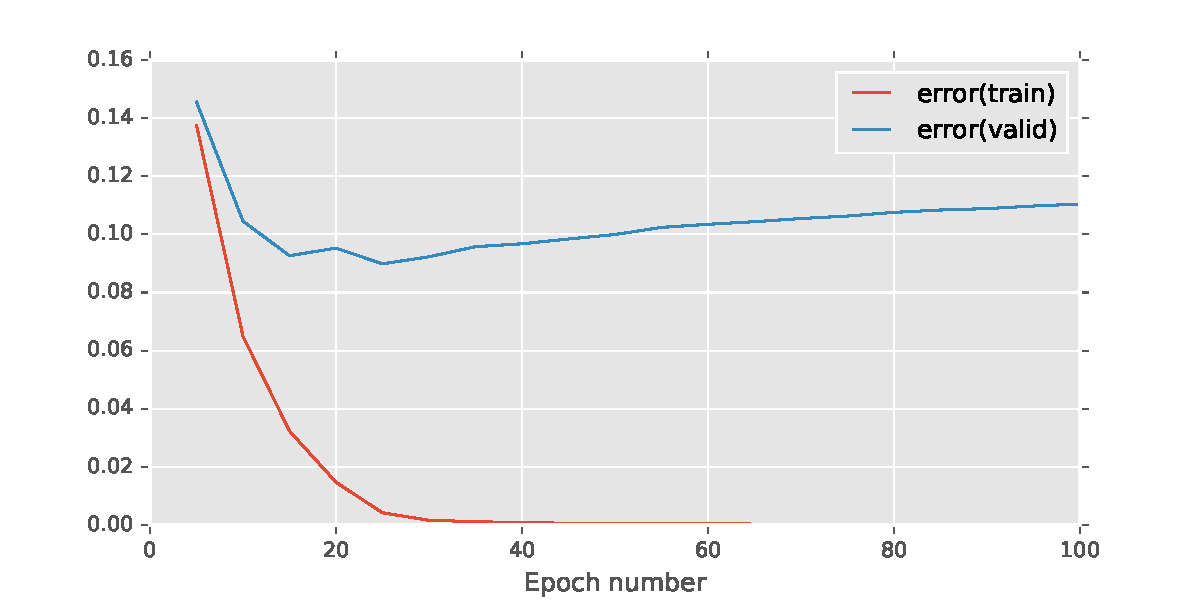
\includegraphics[height=1.5in]{error_with_tau_2_0.pdf}
        \caption{error with $\tau$ = 2.0}
    \end{subfigure}   
    ~
    \begin{subfigure}[t]{0.45\textwidth}
        \centering
        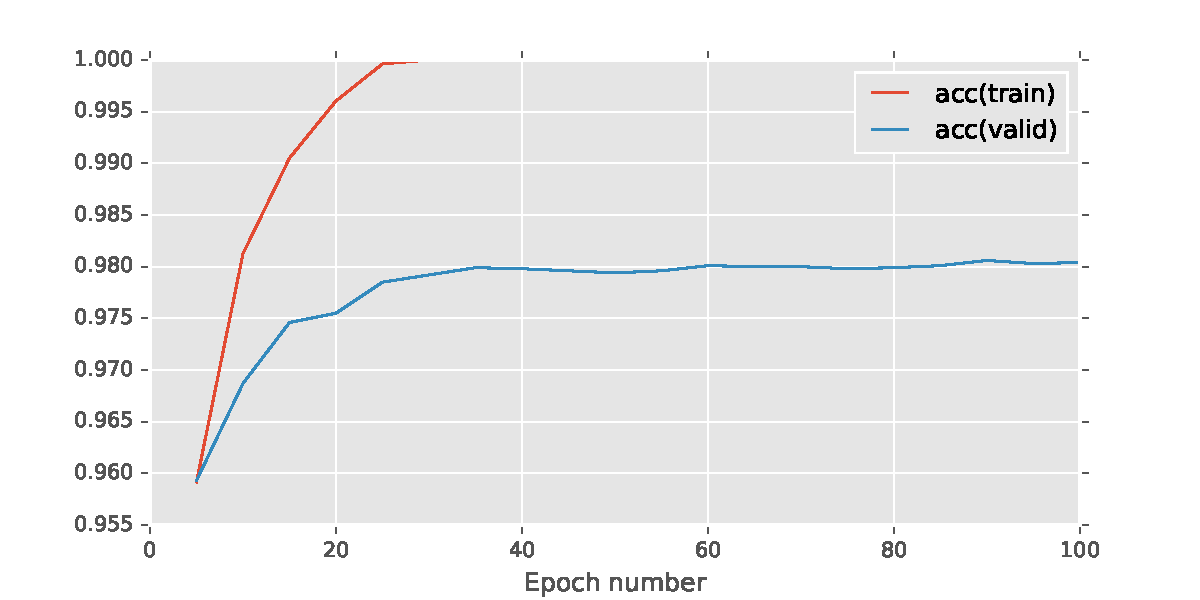
\includegraphics[height=1.5in]{acc_with_tau_2_0.pdf}
        \caption{accuracy with $\tau$ = 2.0}
    \end{subfigure}   
    ~
    \begin{subfigure}[t]{0.45\textwidth}
        \centering
        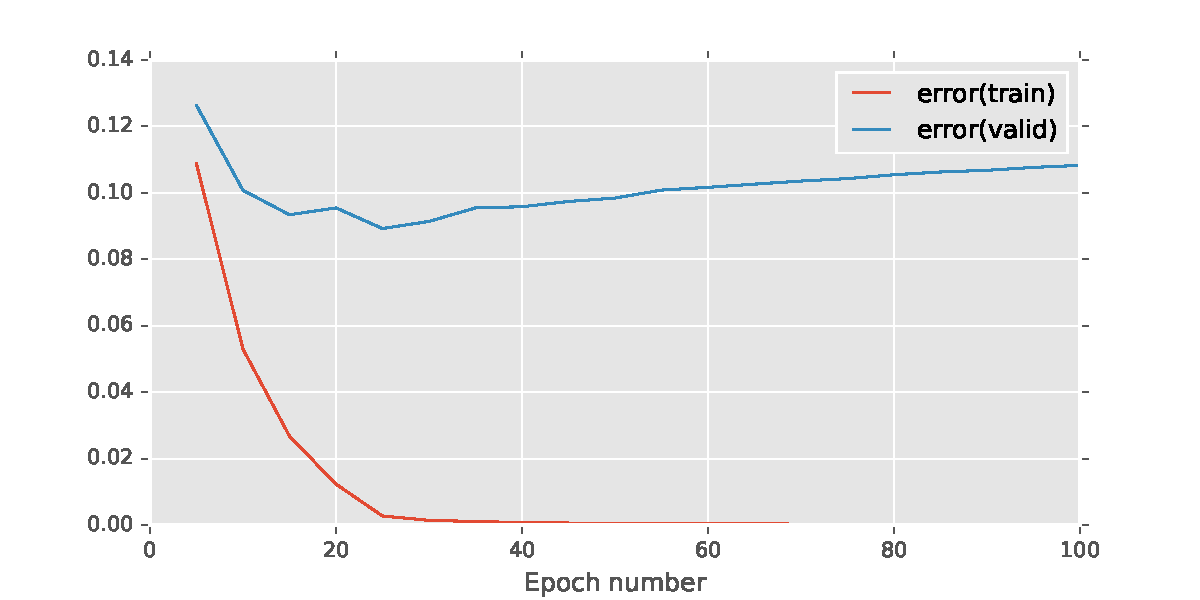
\includegraphics[height=1.5in]{error_with_tau_5_0.pdf}
        \caption{error with $\tau$ = 5.0}
    \end{subfigure}   
    ~
    \begin{subfigure}[t]{0.45\textwidth}
        \centering
        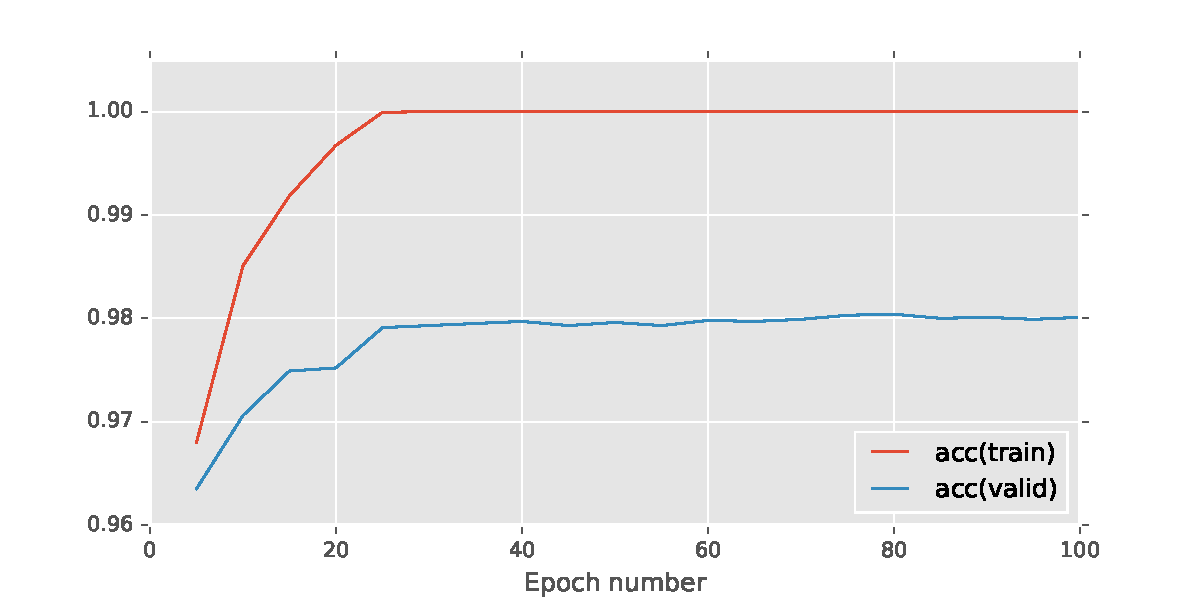
\includegraphics[height=1.5in]{acc_with_tau_5_0.pdf}
        \caption{accuracy with $\tau$ = 5.0}
    \end{subfigure}  
    ~ 
    \begin{subfigure}[t]{0.45\textwidth}
        \centering
        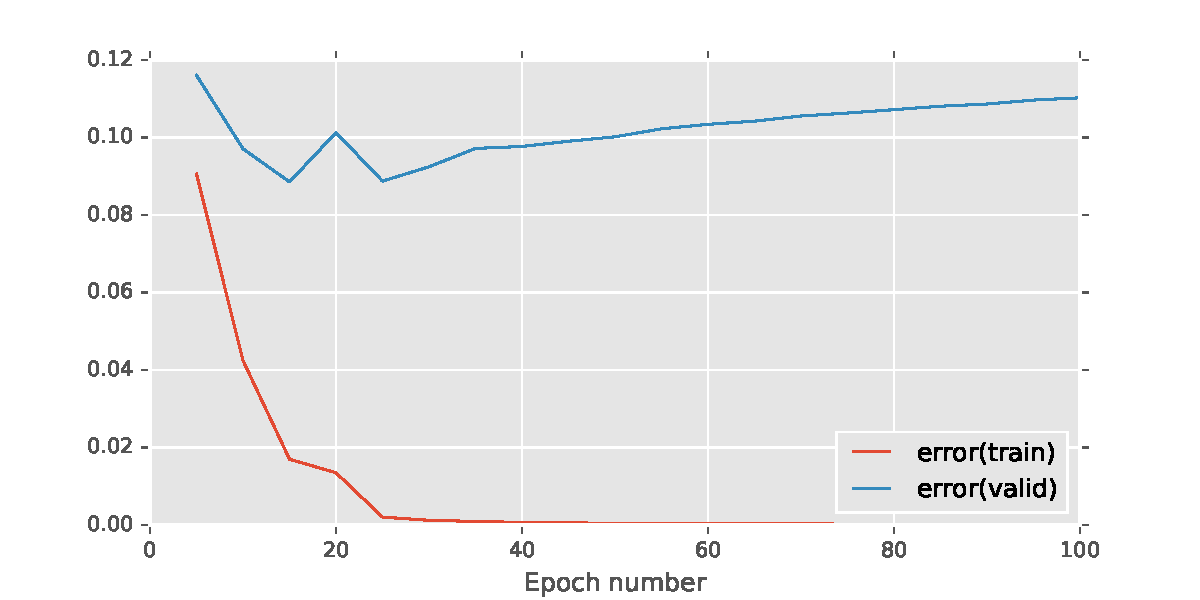
\includegraphics[height=1.5in]{error_with_tau_10_0.pdf}
        \caption{error with $\tau$ = 10.0}
    \end{subfigure}   
    ~
    \begin{subfigure}[t]{0.45\textwidth}
        \centering
        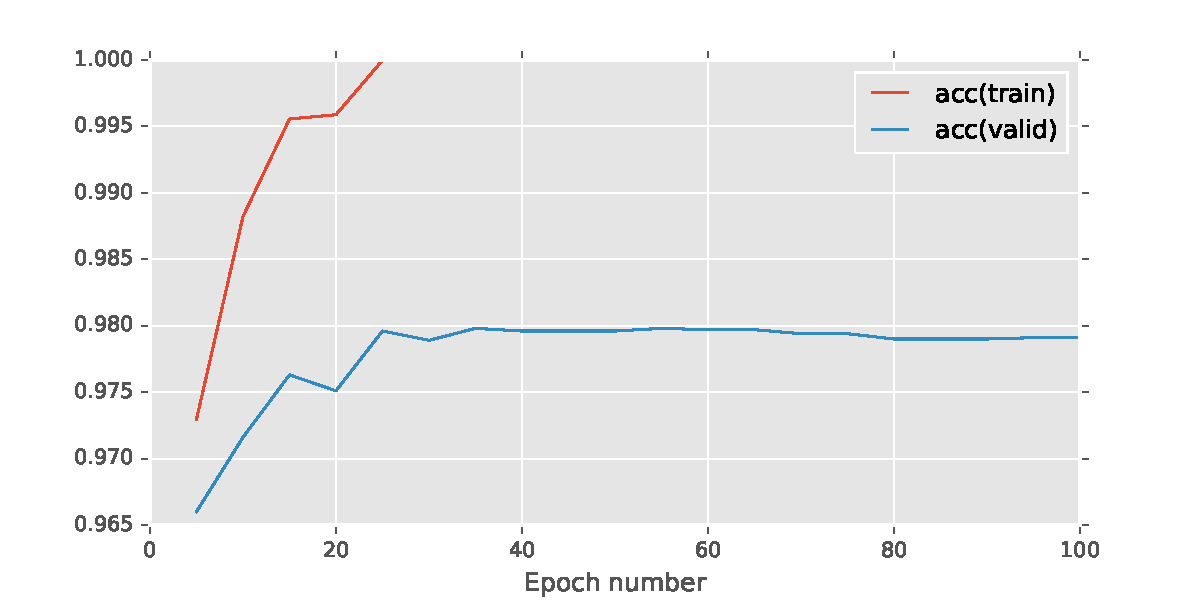
\includegraphics[height=1.5in]{acc_with_tau_10_0.pdf}
        \caption{accuracy with $\tau$ = 10.0}
    \end{subfigure}   
    ~
    \begin{subfigure}[t]{0.45\textwidth}
        \centering
        \includegraphics[height=1.5in]{error_with_tau_100_0.pdf}
        \caption{error with $\tau$ = 100.0}
    \end{subfigure}   
    ~
    \begin{subfigure}[t]{0.45\textwidth}
        \centering
        \includegraphics[height=1.5in]{acc_with_tau_100_0.pdf}
        \caption{accuracy with $\tau$ = 100.0}
    \end{subfigure}   
    \caption{Error and accuracy with several $\tau$ when $\gamma = 1$ using variant momentum coefficient}    
    \label{fig:tau}
\end{figure*}

%Table 7
\begin{table}
\begin{center}
\begin{tabular}{ c c c c c} 
\hline
$\gamma$ & error(train) & error(valid) & acc(train) & acc(valid)\\
\hline
\hline
0.2 & 1.37e-04 & 1.14e-01 & 1.00 & 0.9774 \\ 
0.5 & 1.50e-04 & 1.16e-01 & 1.00 & 0.9785 \\ 
0.7 & 1.59e-04 & 1.13e-01 & 1.00 & 0.9797 \\ 
0.9  &  1.67e-04 & 1.13e-01 & 1.00 & 0.9793 \\
\end{tabular}
\caption{Performance of different $\gamma$ with $\tau$ = 1.0 and asy\_mom\_coeff = 0.9}
\label{tb:tau}
\end{center}	
\end{table}

\begin{figure*}[t!]
    \centering
    \begin{subfigure}[t]{0.45\textwidth}
        \centering
        \includegraphics[height=1.5in]{error_with_gamma_0_2.pdf}
        \caption{error with $\gamma$ = 0.2}
    \end{subfigure}   
    ~
    \begin{subfigure}[t]{0.45\textwidth}
        \centering
        \includegraphics[height=1.5in]{acc_with_gamma_0_2.pdf}
        \caption{accuracy with $\gamma$ = 0.2}
    \end{subfigure}
    ~ 
    \begin{subfigure}[t]{0.45\textwidth}
        \centering
        \includegraphics[height=1.5in]{error_with_gamma_0_5.pdf}
        \caption{error with $\gamma$ = 0.5}
    \end{subfigure}   
    ~
    \begin{subfigure}[t]{0.45\textwidth}
        \centering
        \includegraphics[height=1.5in]{acc_with_gamma_0_5.pdf}
        \caption{accuracy with $\gamma$ = 0.5}
    \end{subfigure}
    ~ 
    \begin{subfigure}[t]{0.45\textwidth}
        \centering
        \includegraphics[height=1.5in]{error_with_gamma_0_7.pdf}
        \caption{error with $\gamma$ = 0.7}
    \end{subfigure}   
    ~
    \begin{subfigure}[t]{0.45\textwidth}
        \centering
        \includegraphics[height=1.5in]{acc_with_gamma_0_7.pdf}
        \caption{accuracy with $\gamma$ = 0.7}
    \end{subfigure}
    ~ 
    \begin{subfigure}[t]{0.45\textwidth}
        \centering
        \includegraphics[height=1.5in]{error_with_gamma_0_9.pdf}
        \caption{error with $\gamma$ = 0.9}
    \end{subfigure}   
    ~
    \begin{subfigure}[t]{0.45\textwidth}
        \centering
        \includegraphics[height=1.5in]{acc_with_gamma_0_9.pdf}
        \caption{accuracy with $\gamma$ = 0.9}
    \end{subfigure}
    \caption{Error and accuracy with several $\gamma$ when $\tau = 1$ using variant momentum coefficient}    
    \label{fig:gamma}
\end{figure*}
 %----------------------------Discussion & Conclusion------------------------------

\subsection{Discussion and Conclusion}
\subsubsection{First task}
Figure \ref{fig:const_mom} indicates that larger momentum coefficient results in a faster convergences and higher speed of learning. Table \ref{tb:mom} indicates that a larger momentum coefficient has larger validation accuracy and smaller train error, which means a better performance. However, the validation error increase when the momentum coefficients increases which indicates overfitting problem.
\subsubsection{Second task}
From Figure \ref{fig:asy_mom}, it can be seen that larger $\alpha_\infty$ results in a faster convergence and its final validation accuracy is similar to smaller $\alpha_\infty$. Table \ref{tb:asy_mom} indicates that the validation error begins to increase when $\alpha_\infty$ increase while the final training error is decreasing. It indicates overfitting problem.

When $\gamma$ is fixed, with the increase of $\tau$, the final training error decreases in the condition that $\tau$ is close to $\gamma$. The higher validation accuracy is achieved when $\tau = 2.0$. Then, with the increase of $\tau$ the validation error increases. In general, The model is not quite sensitive to this parameter.

when $\tau$ is fixed, the system performance is better as $\gamma$ approaching to $\tau$.. When $\gamma$ is very small, the momentum at first epoch is close to asymptotic which is similar to a constant momentum coefficient learning rule. Moreover, the speed of learning rarely changes. 

In conclusion, using a variable momentum coefficient improves the performance over a constant momentum coefficient  baseline according to Table \ref{fig:const_mom}. \ref{fig:asy_mom}. \ref{fig:tau}. and \ref{fig:gamma}.
 %----------------------------Part 3 ------------------------------------------
\newpage
\section{Adaptive learning rules}
In this section, the adaptive learning rules is developed especially the {\bf AdaGrad} and the {\bf RMSProp} which are implemented in the {\bf mlp/learning\_rules.py} module. 
\subsection{Methods and Implementation}
AdaGrad methods is implemented in the method {\bf AdagradLearningRule}. The initial attributes is learning rate and a small constant $\epsilon ~ 10^{-8}$. The update procedure is given by the following equations:
\begin{equation}
	S_i(0) = 0
\end{equation}
\begin{equation}
	S_i(t) = S_i(t-1) + D_i(t)^2
\end{equation}
\begin{equation}
	\Delta w_i(t) = \frac{-\eta }{\sqrt{S_i(t)}+\epsilon }D_i(t)
\end{equation}
$S$ represents sum squared gradient and is represented as {\bf caches} in the method {\bf AdagradLearningRule}. $D_i(t)$ is the gradient of error function $E$ with respect to a weight $W\_i$ at update time $t$. $\Delta w_i(t)$ is the weight change for each echo which is represented as {\bf param} in the code.

Similarly, RMSpropLearingRule is implemented in the method {\bf RMSpropLearningRule} but with one more parameter called decay rate and the implementation of updates is based on the following equations. The main difference is that the RMSProp method replaces the sum by a moving average for $S$.

\begin{equation}
	S_i(t) = \beta S_i(t-1) + (1-\beta)D_i(t)^2
\end{equation}
\begin{equation}
	\Delta w_i(t) = \frac{-\eta }{\sqrt{S_i(t)}+\epsilon }D_i(t)
\end{equation}
$\beta$ is represented as $decay\_rate$ in the method {\bf RMSpropLearningRule}, which is normally $0.9$ as suggested.
%--------------------------Results---------------------------------
\subsection{Results}
The investigation for AdaGrad learning rules is conducted by selecting different values of learning rate. The results is shown in Figure \ref{fig:Adagrad}. and Table \ref{tb:adagrad}.
\begin{figure*}[t!]
    \centering
    \begin{subfigure}[t]{0.45\textwidth}
        \centering
        \includegraphics[height=1.5in]{error_with_Adgrad_0_001.pdf}
        \caption{error for Adgrad with learning rate = 0.001}
    \end{subfigure}   
    ~
    \begin{subfigure}[t]{0.45\textwidth}
        \centering
        \includegraphics[height=1.5in]{acc_with_Adgrad_0_001.pdf}
        \caption{accuracy for Adgrad with learning rate = 0.001}
    \end{subfigure}    
	~
    \begin{subfigure}[t]{0.45\textwidth}
        \centering
        \includegraphics[height=1.5in]{error_with_Adgrad_0_01.pdf}
        \caption{error for Adgrad with learning rate = 0.01}
    \end{subfigure}   
    ~
    \begin{subfigure}[t]{0.45\textwidth}
        \centering
        \includegraphics[height=1.5in]{acc_with_Adgrad_0_01.pdf}
        \caption{accuracy for Adgrad with learning rate = 0.01}
    \end{subfigure}    
	~
    \begin{subfigure}[t]{0.45\textwidth}
        \centering
        \includegraphics[height=1.5in]{error_with_Adgrad_0_05.pdf}
        \caption{error for Adgrad with learning rate = 0.05}
    \end{subfigure}   
    ~
    \begin{subfigure}[t]{0.45\textwidth}
        \centering
        \includegraphics[height=1.5in]{acc_with_Adgrad_0_05.pdf}
        \caption{accuracy for Adgrad with learning rate = 0.05}
    \end{subfigure}    
	~
    \begin{subfigure}[t]{0.45\textwidth}
        \centering
        \includegraphics[height=1.5in]{error_with_Adgrad_0_1.pdf}
        \caption{error for Adgrad with learning rate = 0.1}
    \end{subfigure}   
    ~
    \begin{subfigure}[t]{0.45\textwidth}
        \centering
        \includegraphics[height=1.5in]{acc_with_Adgrad_0_1.pdf}
        \caption{accuracy for Adgrad with learning rate = 0.1}
    \end{subfigure}    
	~
    \begin{subfigure}[t]{0.45\textwidth}
        \centering
        \includegraphics[height=1.5in]{error_with_Adgrad_0_5.pdf}
        \caption{error for Adgrad with learning rate = 0.5}
    \end{subfigure}   
    ~
    \begin{subfigure}[t]{0.45\textwidth}
        \centering
        \includegraphics[height=1.5in]{acc_with_Adgrad_0_5.pdf}
        \caption{accuracy for Adgrad with learning rate = 0.5}
    \end{subfigure}       
    \caption{Error and accuracy using AdaGrad learning rules with several learning rates}    
    \label{fig:Adagrad}
\end{figure*}

%Table 8
\begin{table}
\begin{center}
\begin{tabular}{ c c c c c} 
\hline
Learing Rate & error(train) & error(valid) & acc(train) & acc(valid)\\
\hline
\hline
1e-03 & 3.05e-01 & 2.83e-01 & 0.9163 & 0.9231 \\ 
1e-02 & 5.12e-02 & 9.26e-02 & 0.9863 & 0.9718 \\ 
5e-02 & 6.64e-04 & 9.59e-02 & 1.00 & 0.9799 \\ 
1e-01  &  1.85e-04 & 1.18e-01 & 1.00 & 0.9780 \\
5e-01  &  8.47e-02 & 2.72e-01 & 0.9834 & 0.9453 \\
\end{tabular}
\caption{Performance of different learning rates using AdaGrad Learning rule}
\label{tb:adagrad}
\end{center}	
\end{table}


\begin{figure*}[t!]
    \centering
    \begin{subfigure}[t]{0.45\textwidth}
        \centering
        \includegraphics[height=1.5in]{error_with_RMSprop_0_0001.pdf}
        \caption{error for RMSprop with LR = 0.0001}
    \end{subfigure}   
    ~
    \begin{subfigure}[t]{0.45\textwidth}
        \centering
        \includegraphics[height=1.5in]{acc_with_RMSprop_0_0001.pdf}
        \caption{accuracy for RMSprop with LR = 0.0001}
    \end{subfigure}    
	~
    \begin{subfigure}[t]{0.45\textwidth}
        \centering
        \includegraphics[height=1.5in]{error_with_RMSprop_0_001.pdf}
        \caption{error for RMSprop with LR = 0.001}
    \end{subfigure}   
    ~
    \begin{subfigure}[t]{0.45\textwidth}
        \centering
        \includegraphics[height=1.5in]{acc_with_RMSprop_0_001.pdf}
        \caption{accuracy for RMSprop with LR = 0.001}
    \end{subfigure}    
	~
    \begin{subfigure}[t]{0.45\textwidth}
        \centering
        \includegraphics[height=1.5in]{error_with_RMSprop_0_005.pdf}
        \caption{error for RMSprop with LR = 0.005}
    \end{subfigure}   
    ~
    \begin{subfigure}[t]{0.45\textwidth}
        \centering
        \includegraphics[height=1.5in]{acc_with_RMSprop_0_005.pdf}
        \caption{accuracy for RMSprop with LR = 0.005}
    \end{subfigure}    
	~
    \begin{subfigure}[t]{0.45\textwidth}
        \centering
        \includegraphics[height=1.5in]{error_with_RMSprop_0_01.pdf}
        \caption{error for RMSprop with LR = 0.01}
    \end{subfigure}   
    ~
    \begin{subfigure}[t]{0.45\textwidth}
        \centering
        \includegraphics[height=1.5in]{acc_with_RMSprop_0_01.pdf}
        \caption{accuracy for RMSprop with LR = 0.01}
    \end{subfigure}    
	~
    \begin{subfigure}[t]{0.45\textwidth}
        \centering
        \includegraphics[height=1.5in]{error_with_RMSprop_0_05.pdf}
        \caption{error for RMSprop with LR = 0.05}
    \end{subfigure}   
    ~
    \begin{subfigure}[t]{0.45\textwidth}
        \centering
        \includegraphics[height=1.5in]{acc_with_RMSprop_0_05.pdf}
        \caption{accuracy for RMSprop with LR = 0.05}
    \end{subfigure}       
    \caption{Error and accuracy using RMSprop learning rules with several learning rates}    
    \label{fig:rms}
\end{figure*}

%Table 9
\begin{table}
\begin{center}
\begin{tabular}{ c c c c c} 
\hline
Learing Rate & error(train) & error(valid) & acc(train) & acc(valid)\\
\hline
\hline
1e-04 & 4.13e-02 & 9.23e-02 & 0.9890 & 0.9734 \\ 
1e-03 & 7.41e-08 & 3.14e-01 & 1.0000 & 0.9757 \\ 
5e-03 & 1.62e-04 & 5.04e-01 & 1.0000 & 0.9750 \\ 
1e-02  &  6.38e-03 & 4.90e-01 & 0.9990 & 0.9760 \\
5e-02  &  2.31e-01 & 3.65e-01 & 0.9609 & 0.9520 \\
1e-01  &  4.16e-01 & 4.72e-01 & 0.9278 & 0.9270 \\
\end{tabular}
\caption{Performance of different learning rates using RMSprop Learning rule}
\label{tb:rms}
\end{center}	
\end{table}

Similarly, the effects of learning rates for RMSprop learning rule is given in Figure \ref{fig:rms} and Table \ref{tb:rms}. Additionally, an experiment was conducted to investigate how sensitive to system is to the decay rate $\beta$. The results for different $\beta$ is shown in Figure \ref{fig:rms_decay} and Table \ref{fig:rms_decay}.
\begin{figure*}[t!]
    \centering
    \begin{subfigure}[t]{0.45\textwidth}
        \centering
        \includegraphics[height=1.5in]{error_with_RMSprop_decay_0_1.pdf}
        \caption{error for RMSprop with decay rate = 0.1}
    \end{subfigure}   
    ~
    \begin{subfigure}[t]{0.45\textwidth}
        \centering
        \includegraphics[height=1.5in]{acc_with_RMSprop_decay_0_1.pdf}
        \caption{accuracy for RMSprop with decay rate =  0.1}
    \end{subfigure}    
	~
    \begin{subfigure}[t]{0.45\textwidth}
        \centering
        \includegraphics[height=1.5in]{error_with_RMSprop_decay_0_2.pdf}
        \caption{error for RMSprop with decay rate = 0.2}
    \end{subfigure}   
    ~
    \begin{subfigure}[t]{0.45\textwidth}
        \centering
        \includegraphics[height=1.5in]{acc_with_RMSprop_decay_0_2.pdf}
        \caption{accuracy for RMSprop with decay rate = 0.2}
    \end{subfigure}    
	~
    \begin{subfigure}[t]{0.45\textwidth}
        \centering
        \includegraphics[height=1.5in]{error_with_RMSprop_decay_0_5.pdf}
        \caption{error for RMSprop with decay rate = 0.5}
    \end{subfigure}   
    ~
    \begin{subfigure}[t]{0.45\textwidth}
        \centering
        \includegraphics[height=1.5in]{acc_with_RMSprop_decay_0_5.pdf}
        \caption{accuracy for RMSprop with decay rate = 0.5}
    \end{subfigure}    
	~
    \begin{subfigure}[t]{0.45\textwidth}
        \centering
        \includegraphics[height=1.5in]{error_with_RMSprop_decay_0_9.pdf}
        \caption{error for RMSprop with decay rate = 0.9}
    \end{subfigure}   
    ~
    \begin{subfigure}[t]{0.45\textwidth}
        \centering
        \includegraphics[height=1.5in]{acc_with_RMSprop_decay_0_9.pdf}
        \caption{accuracy for RMSprop with decay rate = 0.9}
    \end{subfigure}    
	~
    \begin{subfigure}[t]{0.45\textwidth}
        \centering
        \includegraphics[height=1.5in]{error_with_RMSprop_decay_0_99.pdf}
        \caption{error for RMSprop with decay rate = 0.99}
    \end{subfigure}   
    ~
    \begin{subfigure}[t]{0.45\textwidth}
        \centering
        \includegraphics[height=1.5in]{acc_with_RMSprop_decay_0_99.pdf}
        \caption{accuracy for RMSprop with decay rate = 0.99}
    \end{subfigure}       
    \caption{Error and accuracy using RMSprop learning rules with several decay rates}    
    \label{fig:rms_decay}
\end{figure*}

%Table 10
\begin{table}
\begin{center}
\begin{tabular}{ c c c c c} 
\hline
decay rate & error(train) & error(valid) & acc(train) & acc(valid)\\
\hline
\hline
0.1 & 2.69e-02 & 7.17-02 & 0.9969 & 0.9643 \\ 
0.2 & 1.06e-02 & 6.07e-01 & 0.9986 & 0.9683 \\ 
0.5 & 5.57e-05 & 6.41e-01 & 1.0000 & 0.9697 \\ 
0.9  &  1.62e-04 & 5.04e-01 & 1.0000 & 0.9750 \\
0.99  &  1.19e-03 & 2.72e-01 & 0.9996 & 0.9767 \\
\end{tabular}
\caption{Performance of different decay rates using RMSprop learning rule}
\label{tb:rms_decay}
\end{center}	
\end{table}

\subsection{Discussion and Conclusion}
\subsubsection{AdaGrad}
For AdaGrad learning rules, except for large learning rules (over $0.5$) or small learning rules (below $0.01$) the speed of convergence is the highest with a good performance. Moreover, the validation error starts to increase while the training error is decrease when learning rate increases which suggests the model is overfitting to the data. one possible of drawback could be that the learning stops too early 
\subsubsection{RMSprop}
The RMSprop learning rules is unstable during converges suggesting a large step size. Although providing with good speed of convergence, the model using RMSprop learning rules reaches its convergence very early but is quite unstable during the later training. Also, the model is not overfitting when the learning rate is $1e-4$. For higher learning rate, the model starts to overfit the training data. Interestingly, when leaning rate = 0.05, the trend of validation error follows the training error. However, the system is quite unstable. This is probably because of the large step size prevents the model from overfitting.

Increasing decay rates results in a better final accuracy on validation. However, the training error increases after decay rate increases over 0.5. However, in general, the system is not very sensitive to decay rate. From the plots, the rends are similar for different values of decay rates. In summary, a high decay rate is suggested to achieve better performance. 

\subsubsection{Comparison}
The comparison of performance in terms speed of convergence and the final error / accuracy on both training and validation data sets. The Table \ref{tb:final_P} shows the results including final error and classification accuracy for both training and validation data sets, run time per epoch, free parameters set for different learning rules, where LR represents learning rates, Mom represents momentum coefficient and 
For AdaGrad, RMSprop, basic gradient descent and momentum learning rules. The speed of convergence from high to low is: AdaGrad, RMSprop, momentum learning and basic gradient descent. 

For the training error, the adaptive learning rules have better results. However, they are not as good as basic gradient descent learning rules in terms of validation error. This suggests a overfitting problem. Early stop may be a solution to overcome overfitting.
All of four models have similar results in accuracy. However, the final accuracy of RMSprop is not the best results during the entire epochs probability because of its instability.

In terms of run time per epoch, applying adaptive learning rules is more time-consuming than the basic gradient descent or momentum learning rules. It should be cared to choose adaptive learning rules if the computational resources is limited. 



%Table 10
\begin{table}
\begin{center}
\begin{tabular}{ c c c c c c c} 
\hline
learning rules & free params & error(train) & error(valid) & acc(train) & acc(valid) & run time/epoch\\
\hline
\hline
Basic 		&  LR =	0.1				&  5.64e-03 & 8.92e-02 & 1.00 & 9.77e-01 & 1.10s\\ 
Momentum 	& LR 0.1, Mom = 0.9		&  1.28e-04 & 1.13e-01 & 1.00 & 0.9787 & 1.26s\\
AdaGrad		& LR = 0.1,	$\beta$= 0.9&1.85e-04 	& 1.18e-01 & 1.00 & 0.9780 &  2.09s\\ 
RMSprop 	& LR = 5e-03 			& 1.62e-04  & 5.04e-01 & 1.00 & 0.9750 & 2.05s\\
\end{tabular}
\caption{Overall Performance of different learning rules}
\label{tb:final_P}
\end{center}	
\end{table}

\end{document}
